%% The following is a directive for TeXShop to indicate the main file
%%!TEX root = diss.tex

\chapter{Results}
\label{ch:Results}

In this chapter we show results for the \hyperref[sec:BDI]{BDI}, \hyperref[sec:Dedup]{Dedup}, and \hyperref[sec:Final Implementation]{DedupBDI} caches along with the \hyperref[sec:Upper Bound]{roofline model} we established for DedepBDI. We show how those four cache designs affect compression, MPKI, and speedup.

\section{Methodology}
\label{sec:Methodology}
\begin{table}[]
    \centering
    \begin{tabular}{ll}
        Component & Configuration                                                                                                                                            \\ \hline
        CPU       & x86\_64, 2.6GHz, 4-wide OoO, 80 entry ROB.                                                                                                               \\
        L1I       & 32KB, 4 way, 3 cycle access lat, 64B lines, LRU.                                                                                                         \\
        L1D       & 32KB, 8 way, 4 cycle access lat, 64B lines, LRU.                                                                                                         \\
        L2        & Private, 256KB, 8 way, 11 cycle access lat, 64B lines, LRU.                                                                                              \\
        L3        & \begin{tabular}[c]{@{}l@{}}Shared, 0.5MB-8MB (or similar tag array size if compressed),\\  16 way, 39 cycle access lat, 64B lines, 8 banks.\end{tabular} \\
        Mem       & DDR3-1066, 1GB.                                                                                                                                         
        \end{tabular}
    \caption{The simulated system}
    \label{tab:simsys}
\end{table}
\begin{table}[]
    \centering
    \begin{tabular}{|l|l|l|l|}
    \hline
    Compression                   & Cache & Data Entries & Tag Entries \\ \hline
    \multirow{5}{*}{Conventional} & 0.5MB & 8192         & 8192        \\ \cline{2-4} 
                                  & 1MB   & 16384        & 16384       \\ \cline{2-4} 
                                  & 2MB   & 32768        & 32768       \\ \cline{2-4} 
                                  & 4MB   & 65536        & 65536       \\ \cline{2-4} 
                                  & 8MB   & 131072       & 131072      \\ \hline
    \multirow{5}{*}{COMP-2}       & 0.5MB & 4096         & 8192        \\ \cline{2-4} 
                                  & 1MB   & 8192         & 16384       \\ \cline{2-4} 
                                  & 2MB   & 16384        & 32768       \\ \cline{2-4} 
                                  & 4MB   & 32768        & 65536       \\ \cline{2-4} 
                                  & 8MB   & 65536        & 131072      \\ \hline
    \multirow{5}{*}{COMP-4}       & 0.5MB & 2048         & 8192        \\ \cline{2-4} 
                                  & 1MB   & 4096         & 16384       \\ \cline{2-4} 
                                  & 2MB   & 8192         & 32768       \\ \cline{2-4} 
                                  & 4MB   & 16384        & 65536       \\ \cline{2-4} 
                                  & 8MB   & 32768        & 131072      \\ \hline
    \end{tabular}
    \caption{All cache configurations.}
    \label{tab:simcache}
\end{table}
We used the zsim\cite{zsim} simulator to design and implement the four target caches: BDI, Dedup, DedupBDI, and Ideal DedupBDI along with a baseline conventional (uncompressed) cache. We used an out-of-order core timing model based on a medium-size x86 core, with detailed timing for all critical-path and off-critical-path events. We simulated a system with a 3 level cache hierarchy, with private L1 and L2 caches and a shared L3 cache. The simulated system is listed in Table \ref{tab:simsys}.\par 
We simulated different conventional L3 cache sizes ranging from 0.5MB to 8MB. We also simulated the four compressed caches at the same tag array sizes, but with data arrays half and one quarter of the size. For example, a 4MB-2 BDI cache has the same number of tags as a conventional 4MB cache, but its tag to data ratio is 2 so its data array size is half of its conventional counterpart. The LLC cache configurations are shown in \ref{tab:simcache}. The workloads used are all the benchmarks from the AxBench\cite{axbench} benchmark suite, the Parsec\cite{parsec} benchmark suite with simmedium inputs, and the Spec\cite{spec} benchmark suite with train inputs (mid-size inputs). All the benchmarks were simulated until end or 3 billion instructions.

\section{Case Study}
\label{sec:case_study}
In this section we describe the four benchmarks we picked in \ref{sec:Motivation}. The benchmarks have different cache patterns and behaviors. During the static analysis done in \ref{sec:Motivation} canneal was only compressible by BDI, dedup was compressible using deduplication, jmeint was uncompressible while libquantum was compressible by both. We analyze how these benchmarks behave when simulated in a real computing system with compressed caches.\par
\begin{figure}
    \begin{subfigure}{\textwidth}
        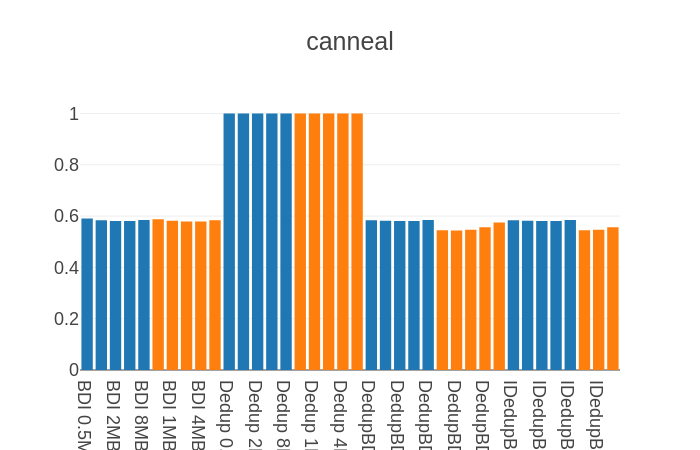
\includegraphics[width=\textwidth]{canneal-compratio.png}
        \caption{canneal}
    \end{subfigure}
    \begin{subfigure}{\textwidth}
        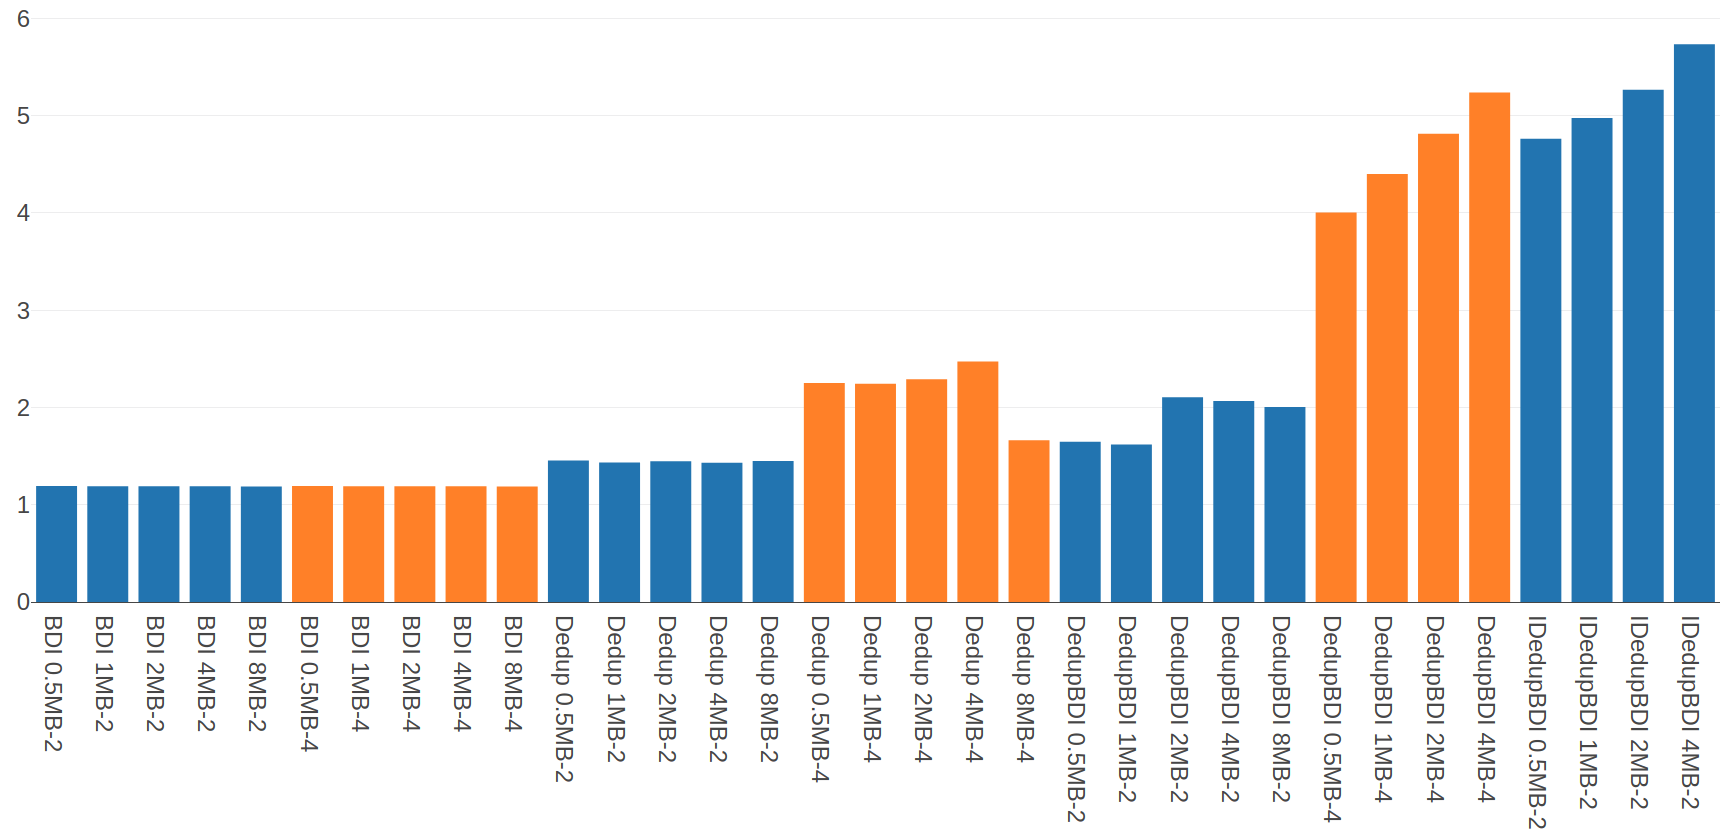
\includegraphics[width=\textwidth]{lbm-compratio.png}
        \caption{lbm}
    \end{subfigure}
    \caption[Case Study: Compression1]{Showing four benchmarks and their compression ratio using different compressed caches.}
    \label{fig:case_compratio1}
\end{figure}
\begin{figure}
    \begin{subfigure}{\textwidth}
        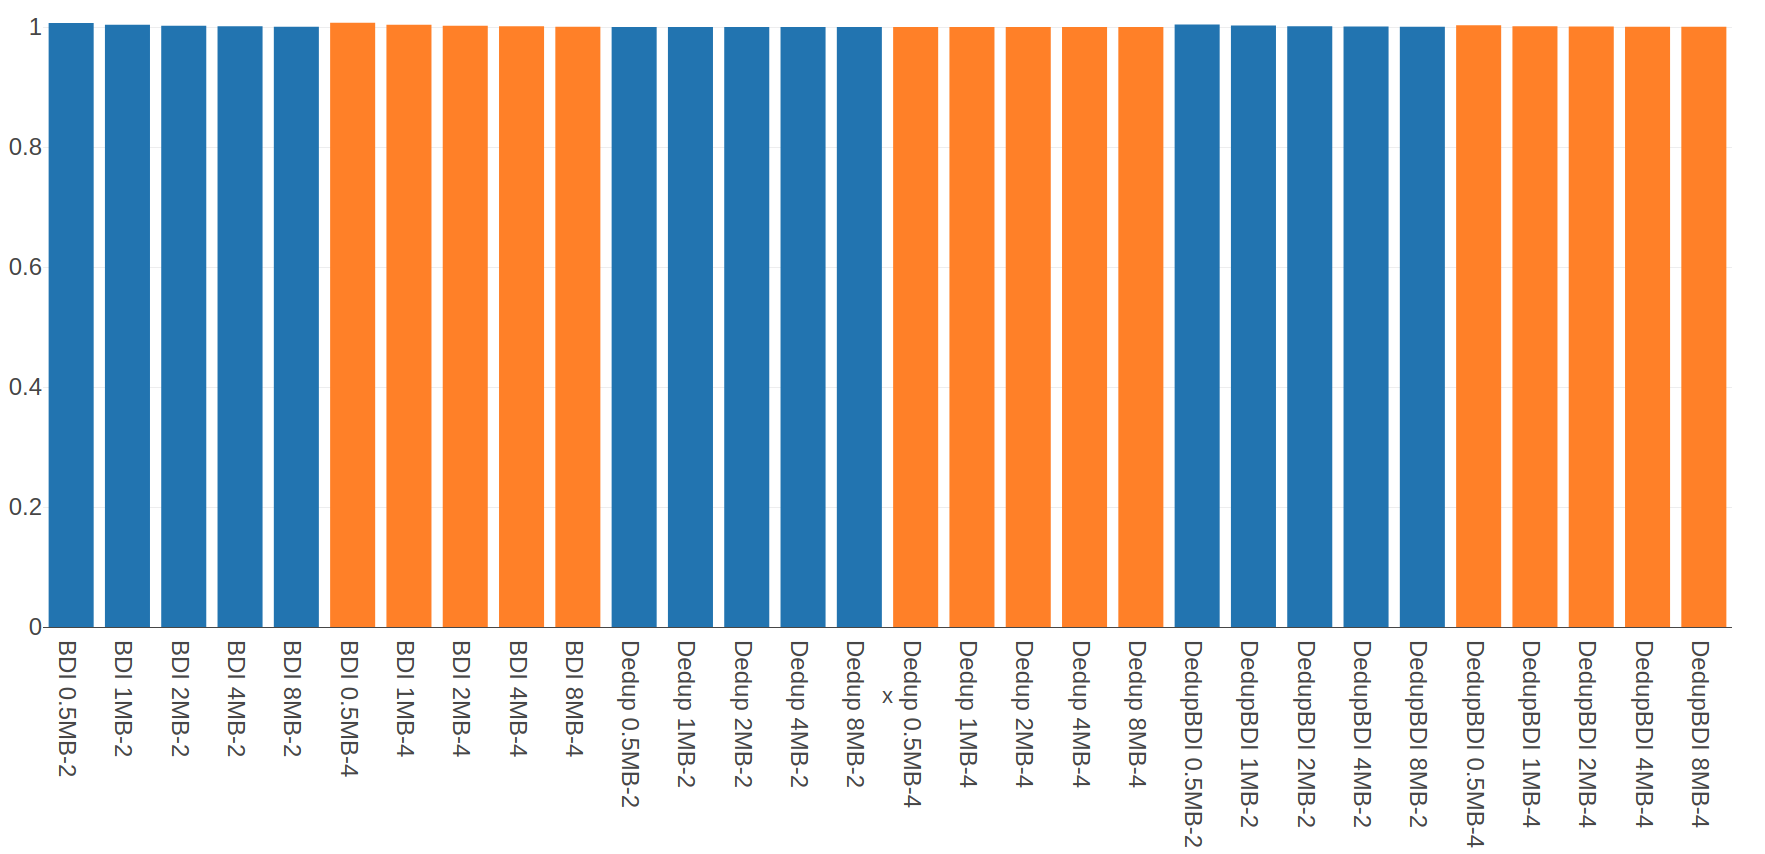
\includegraphics[width=\textwidth]{jmeint-compratio.png}
        \caption{jmeint}
    \end{subfigure}
    \begin{subfigure}{\textwidth}
        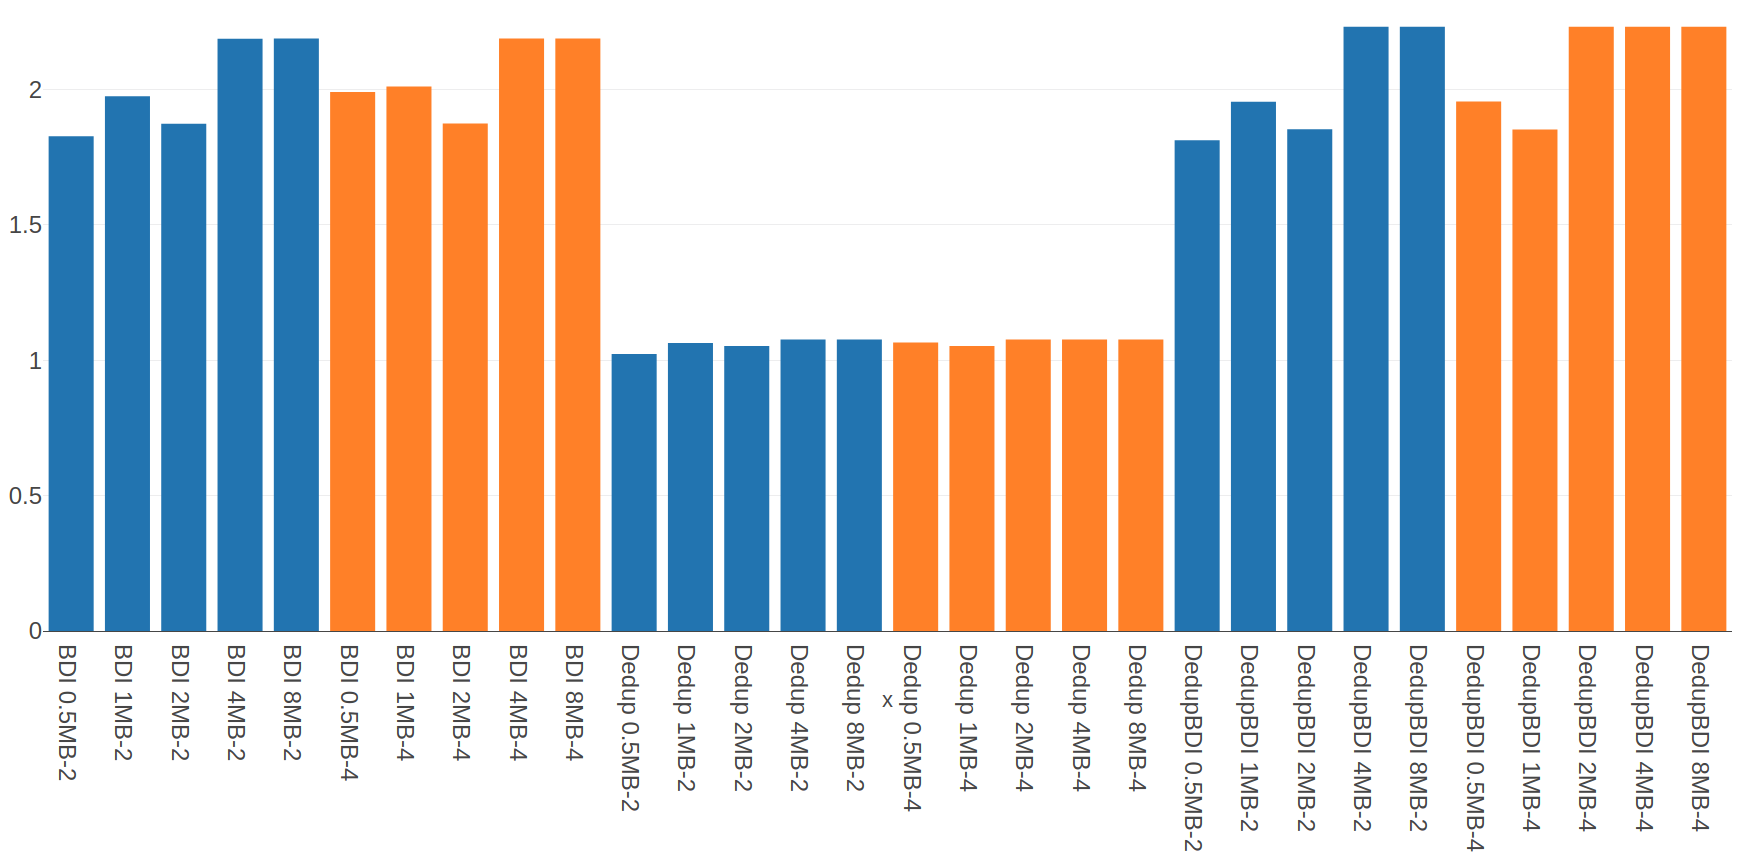
\includegraphics[width=\textwidth]{libquantum-compratio.png}
        \caption{libquantum}
    \end{subfigure}
    \caption[Case Study: Compression2]{Showing four benchmarks and their compression ratio using different compressed caches.}
    \label{fig:case_compratio2}
\end{figure}
\begin{figure}
    \begin{subfigure}{0.5\textwidth}
        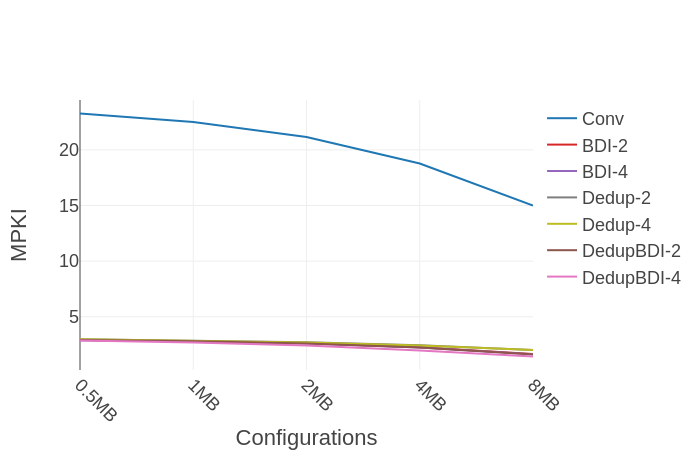
\includegraphics[width=\textwidth]{canneal-mpki.png}
        \caption{canneal}
    \end{subfigure}
    \begin{subfigure}{0.5\textwidth}
        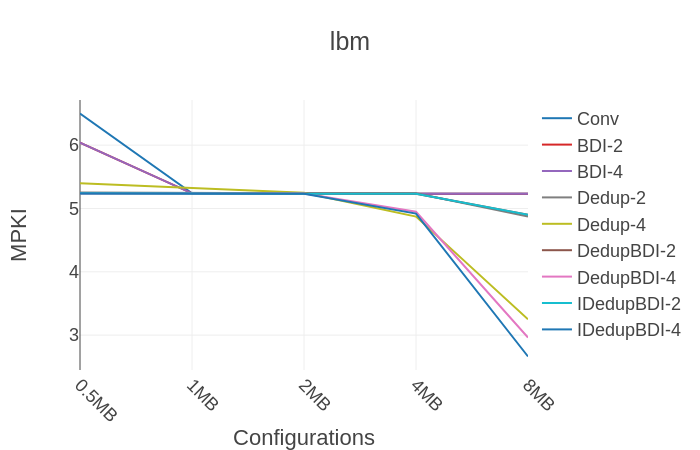
\includegraphics[width=\textwidth]{lbm-mpki.png}
        \caption{lbm}
    \end{subfigure}
    \begin{subfigure}{0.5\textwidth}
        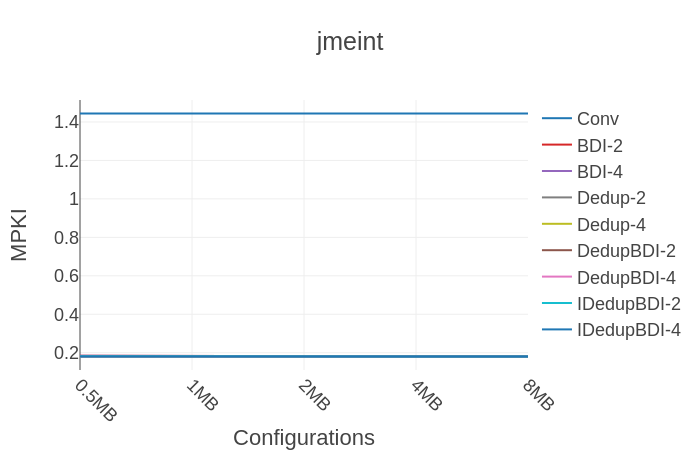
\includegraphics[width=\textwidth]{jmeint-mpki.png}
        \caption{jmeint}
    \end{subfigure}
    \begin{subfigure}{0.5\textwidth}
        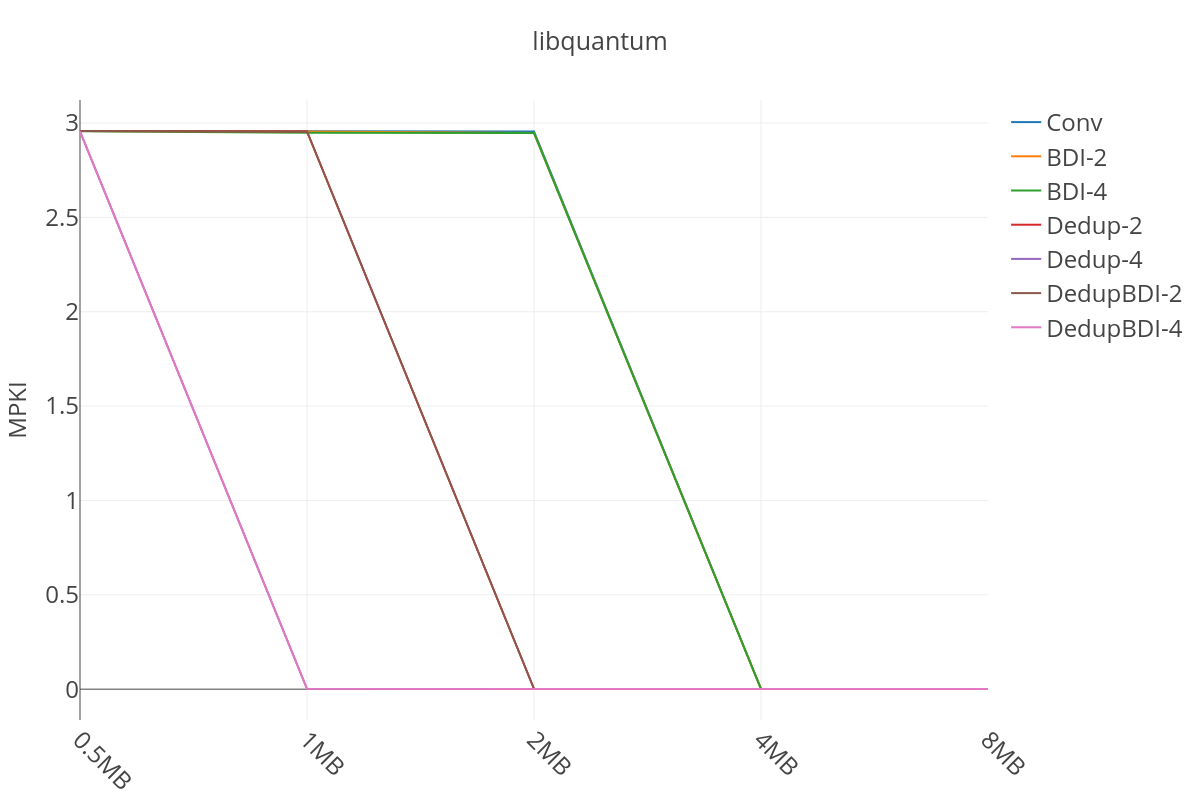
\includegraphics[width=\textwidth]{libquantum-mpki.png}
        \caption{libquantum}
    \end{subfigure}
    \caption[Case Study: MPKI]{Showing four benchmarks and their MPKI using different compressed caches.}
    \label{fig:case_mpki}
\end{figure}
\begin{figure}
    \begin{subfigure}{0.5\textwidth}
        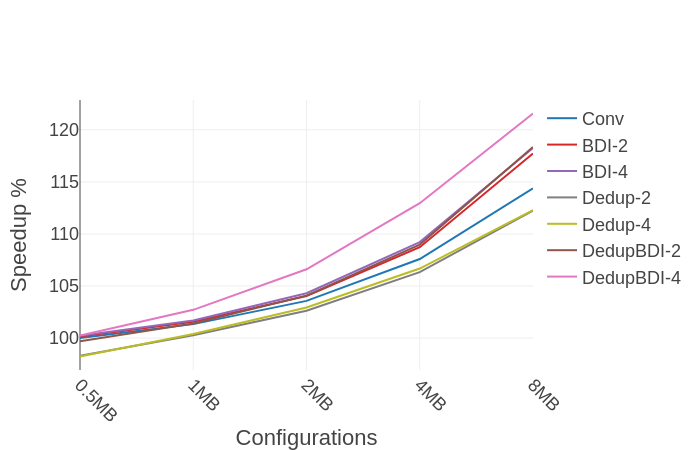
\includegraphics[width=\textwidth]{canneal-speedup.png}
        \caption{canneal}
    \end{subfigure}
    \begin{subfigure}{0.5\textwidth}
        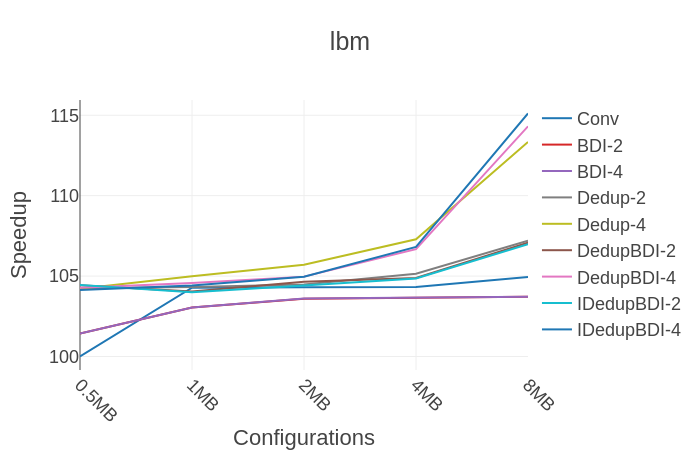
\includegraphics[width=\textwidth]{lbm-speedup.png}
        \caption{lbm}
    \end{subfigure}
    \begin{subfigure}{0.5\textwidth}
        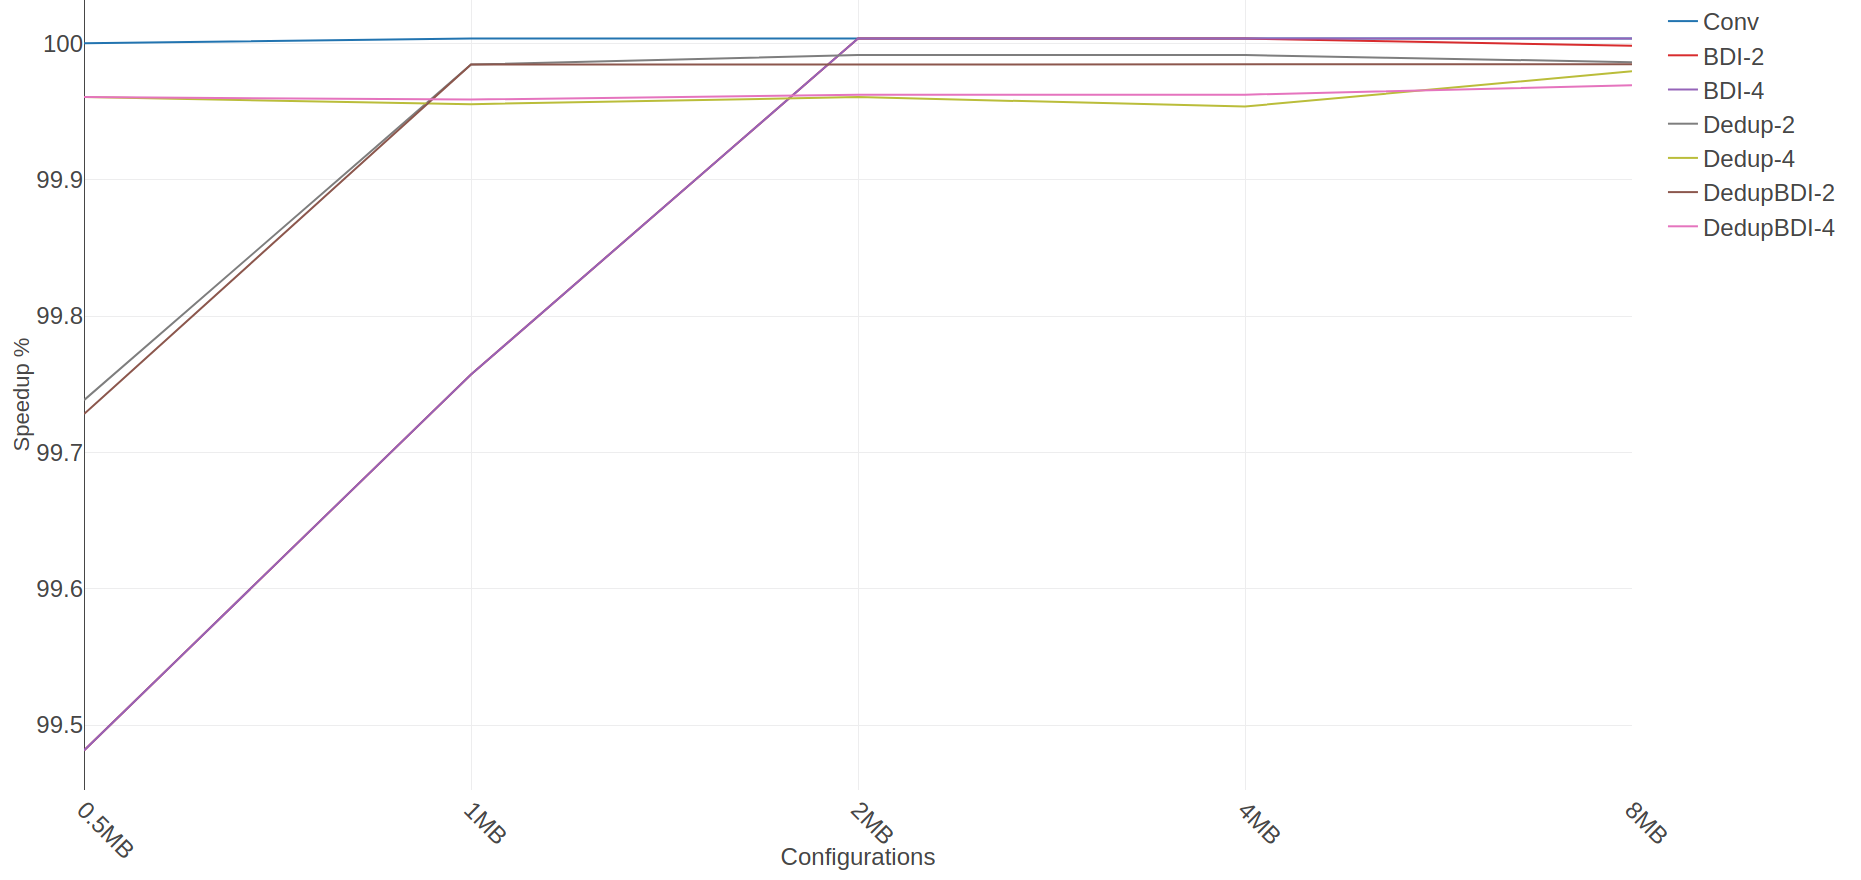
\includegraphics[width=\textwidth]{jmeint-speedup.png}
        \caption{jmeint}
    \end{subfigure}
    \begin{subfigure}{0.5\textwidth}
        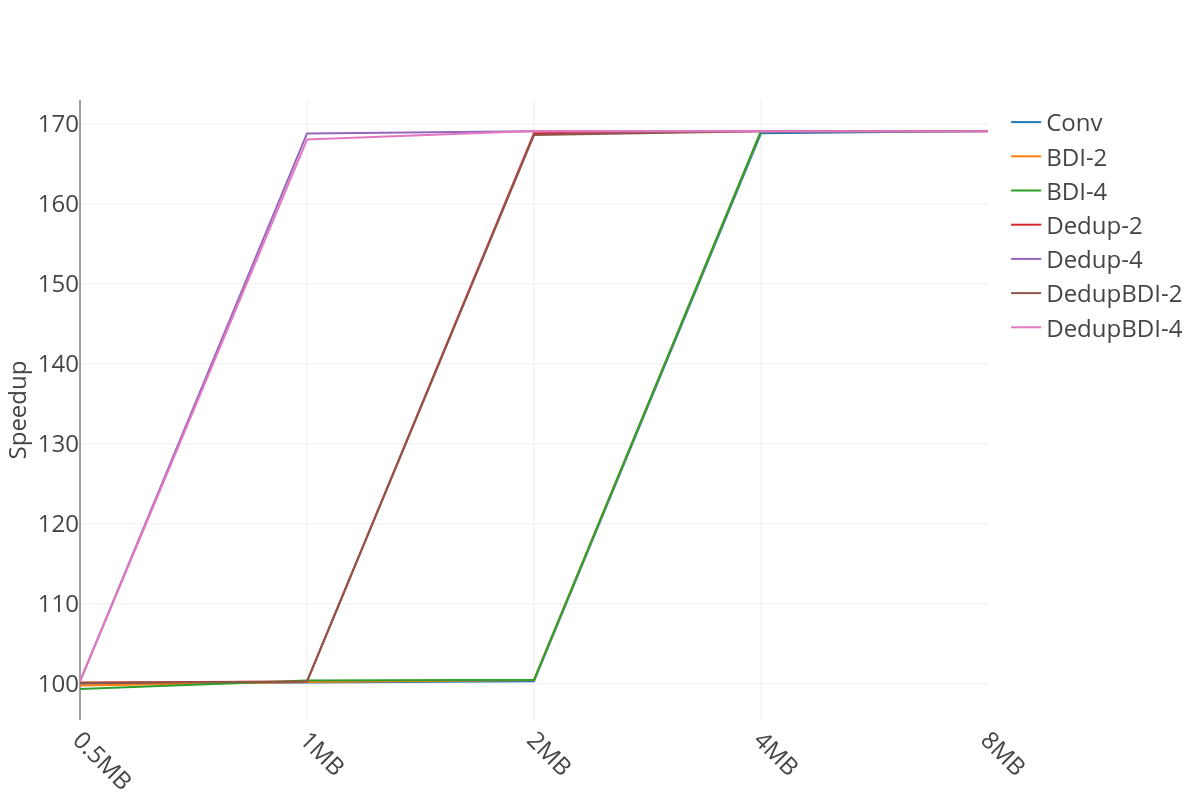
\includegraphics[width=\textwidth]{libquantum-speedup.png}
        \caption{libquantum}
    \end{subfigure}
    \caption[Case Study: Speedup]{Showing four benchmarks and their speedup using different compressed caches.}
    \label{fig:case_speedup}
\end{figure}
Figures \ref{fig:case_compratio1} and \ref{fig:case_compratio2} show the compression ratio of the four benchmarks. Compression ratio is calculated as the ratio between valid tags and valid data entries. The blue columns are caches with tag entries double the data entries, while the orange ones have tags four times the data entries. As expected, canneal shows some compression with BDI but nothing with Dedup, lbm shows compression using Dedup but not using BDI, jmeint shows no compression using any of the caches, while libquantum shows compression using all of them. The DedupBDI cache combines the best of both worlds and either outperforms or at least does as good as BDI or Dedup.\par
Figures \ref{fig:case_mpki} and \ref{fig:case_speedup} show the MPKI and Speedup for the four benchmarks under all cache configurations. Apart from the incompressible jmeint, all the benchmarks show big speedups (up to 70\% in case of libquantum). DedupBDI is the best performing cache in canneal, lbm and libquantum. But it's slightly worse (0.05\% slowdown) than a conventional cache in jmeint.\par
This shows how the DedupBDI cache brings together the best of both worlds. It is able to function exactly similar to BDI and Dedup in cases that are only compressible by one, and it is able to use both compressions at the same time to enhance compression and performance. Although the cost for this is its increased complexity and access latency that causes it to perform slightly worse in incompressible cases.

\section{Compression}
\label{sec:Compression}
Figure \ref{fig:all_compratio} shows the compression ratio for all the benchmarks when simulated with a compressed 4MB LLC with tags four times the data lines. It's shown that DedupBDI performs either better than BDI and Dedup, or at least similar to the dominant one. There're no cases in which DedupBDI compressed worse than BDI or Dedup.\par
It can also be seen that the difference between DedupBDI and the roofline model (IDedupBDI) is minimal in most cases. Only in bwaves and fft benchmarks the roofline perform a lot better than the real world implementation.\par
However, the compression ratio does not tell the full story. If a cache contains 512 valid tags out of 1024, and 256 valid data lines out of 256 then it has a compression ratio of 0.5 but it's not being fully utilized. Normal conventional caches usually have near 100\% utilization unless the working data set is very small to entirely fit inside a cache. Figure \ref{fig:all_util} shows the tag and data array utilization for all benchmarks. Most of the benchmarks can be divided into two categories:
\begin{itemize}
    \item \textbf{tag limited:} Those are benchmarks that have very high tag utilization, but lower than 100\% data utilization. GemsFDTD is an obvious example. Those benchmarks are highly compressible and thus are bound by the size of the tag array. Evictions in such benchmarks are mainly caused by the tag array replacement policy.
    \item \textbf{data limited:} Those benchmarks reach 100\% utilization of their data arrays before the tag array is full. This is because they have a lower degree of compressibility. Evictions in those benchmarks are prominently caused by the data array replacement policy.
\end{itemize}
\begin{figure}
    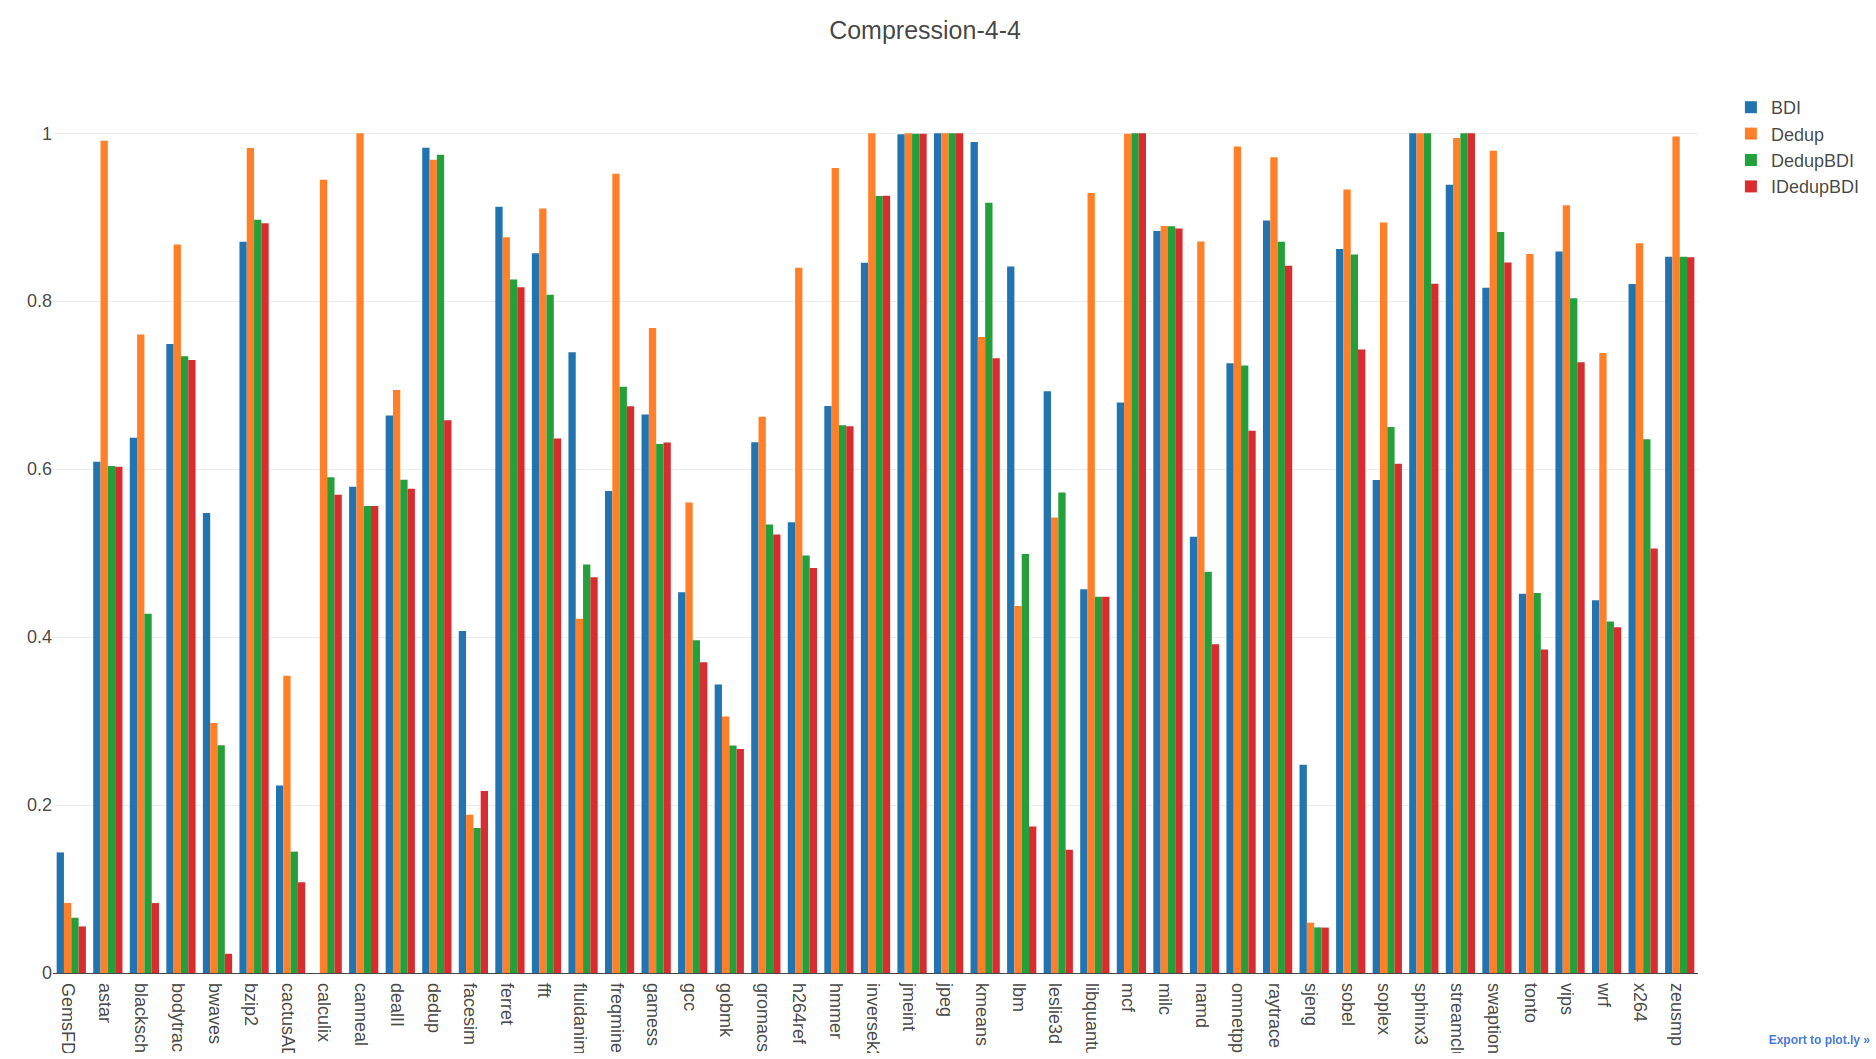
\includegraphics[width=\textwidth]{all-compratio.png}
    \caption[All benchmarks: Compression]{Showing compression ratio for all benchmarks using all types of compressed 4MB caches with tags four times data.}
    \label{fig:all_compratio}
\end{figure}
\begin{figure}
    \begin{subfigure}{\textwidth}
        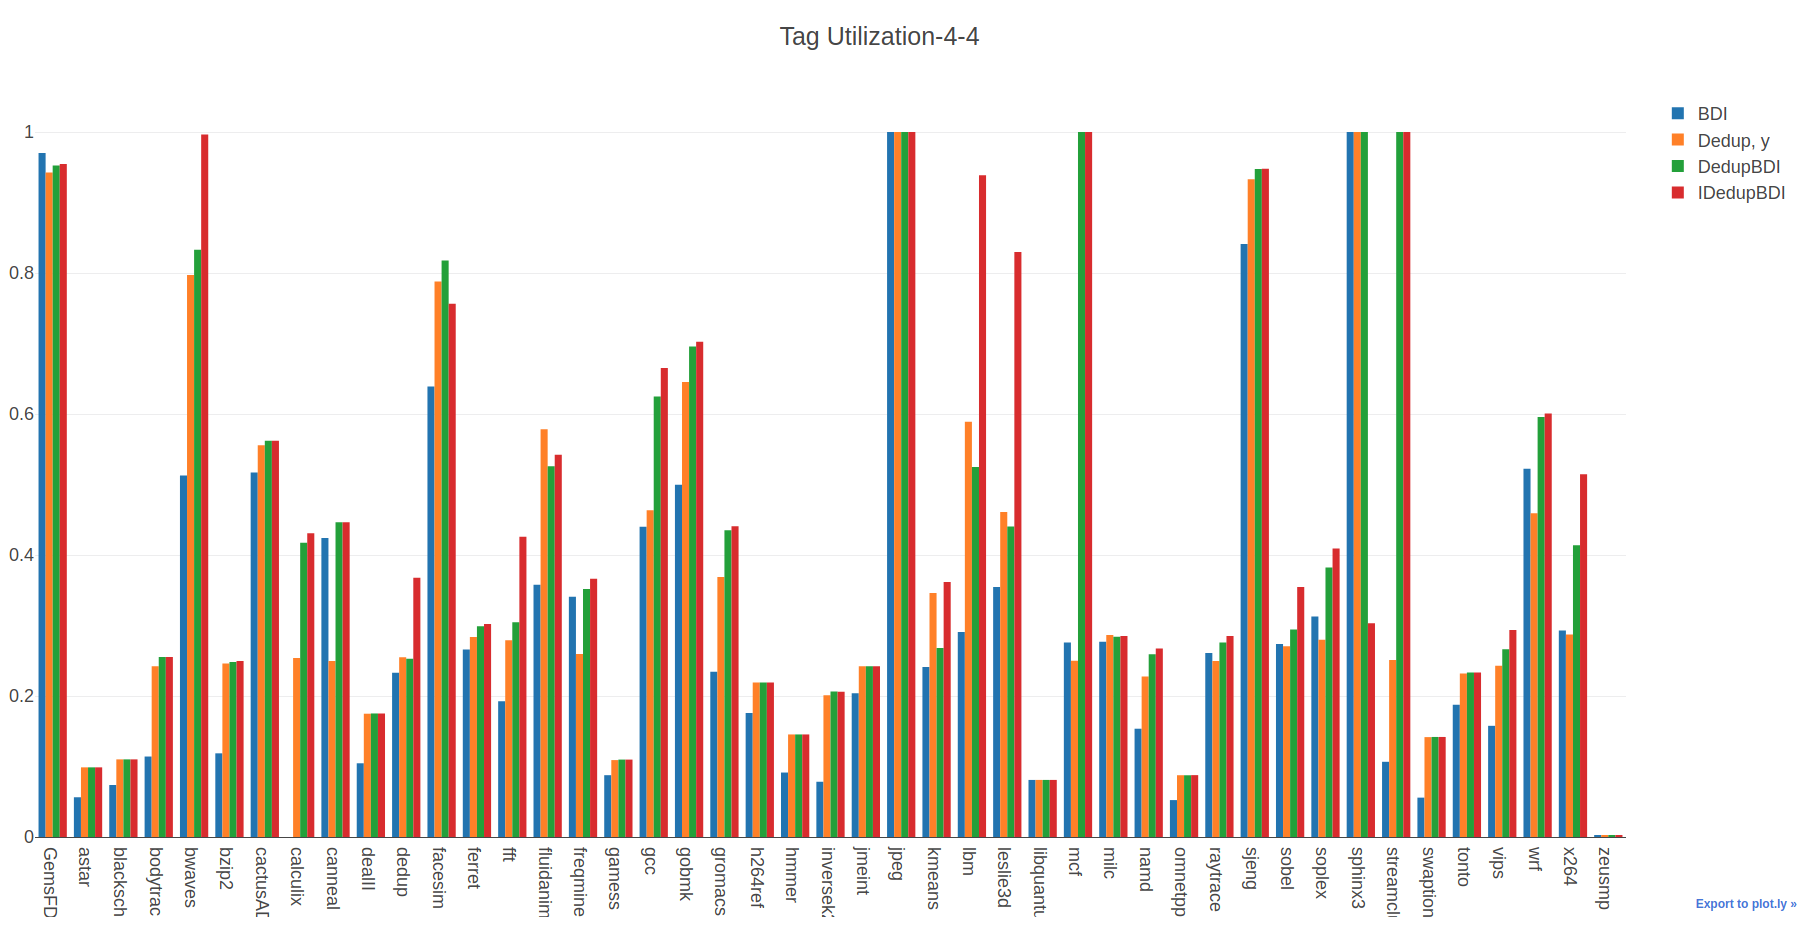
\includegraphics[width=\textwidth]{all-tagutil.png}
    \end{subfigure}
    \begin{subfigure}{\textwidth}
        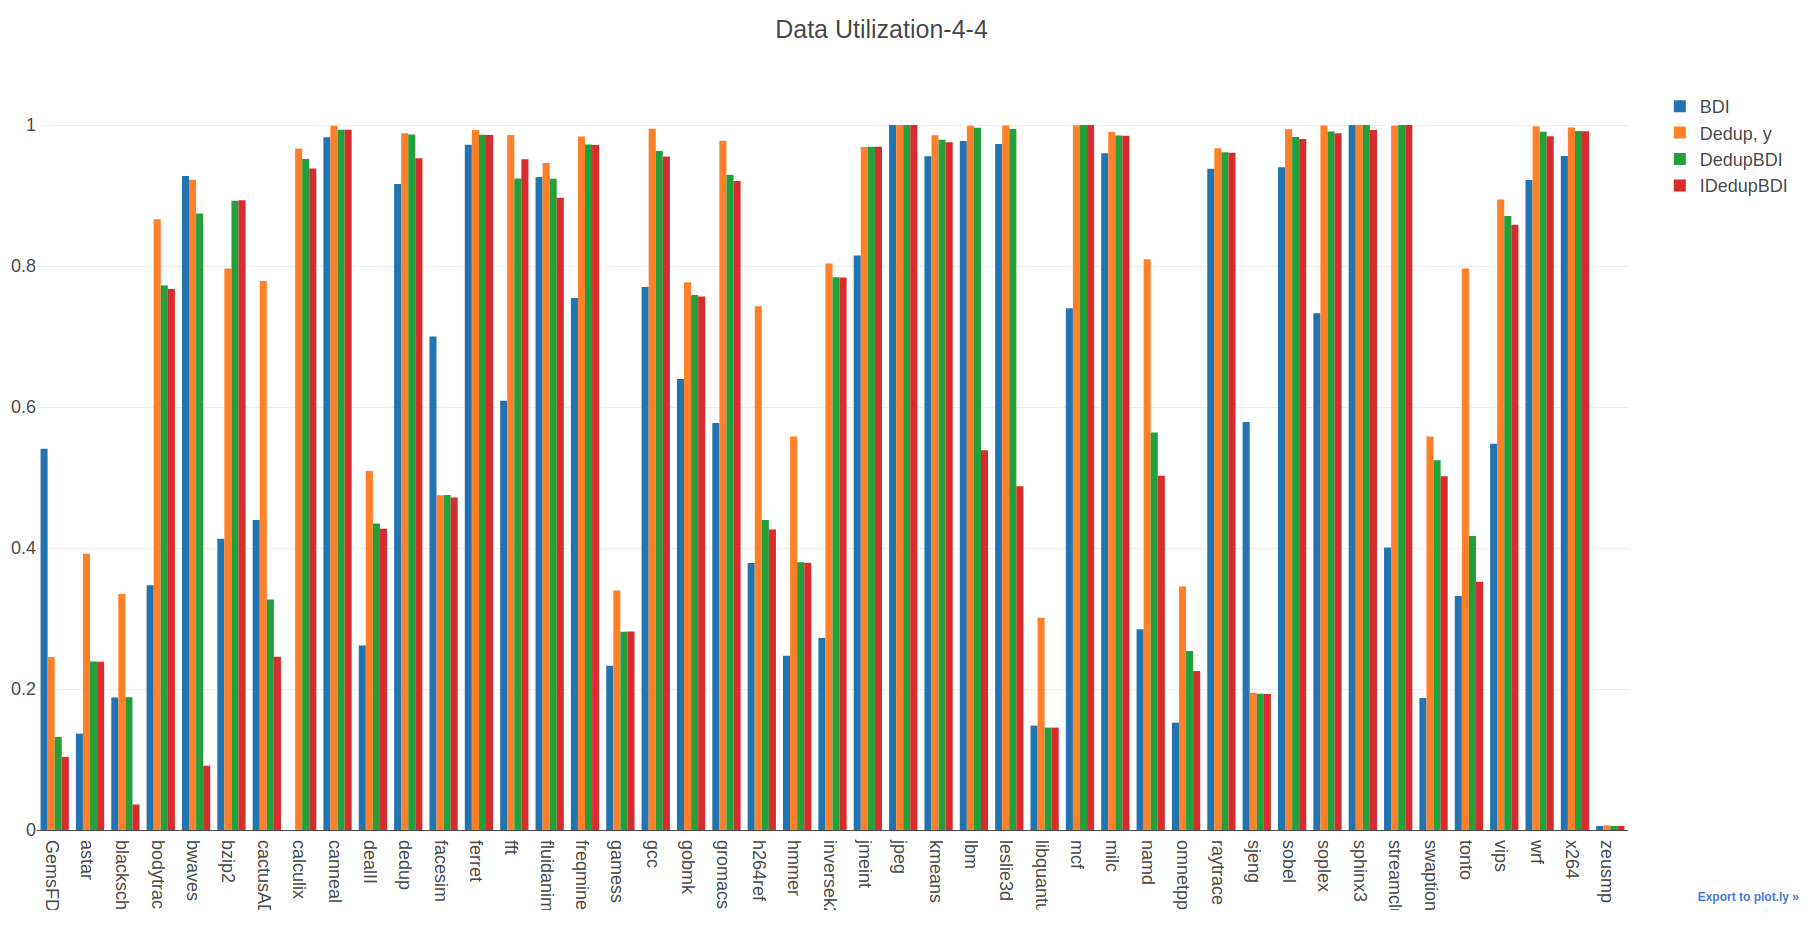
\includegraphics[width=\textwidth]{all-datautil.png}
    \end{subfigure}
    \caption[All benchmarks: Utilization]{Showing tag and data utilization ratio for all benchmarks using all types of compressed 4MB caches with tags four times data.}
    \label{fig:all_util}
\end{figure}
Results generated from other cache sizes (ranging from 0.5MB to 8MB) are very similar, we have chosen the 4MB-4 as a representative.

\section{Performance}
\label{sec:Performance}
\begin{table}[]
    \centering
    \small
    \setlength\tabcolsep{2pt}
    \begin{tabular}{|l|l|l|l|l|l|l|l|}
        \hline
        \textbf{Benchmark} & \textbf{Cache Sensitive}                                    & \textbf{Benchmark} & \textbf{Cache Sensitive}                                      & \textbf{Benchmark} & \textbf{Cache Sensitive}                                     & \textbf{Benchmark} & \textbf{Cache Sensitive}                                      \\ \hline
        fft                & \begin{tabular}[c]{@{}l@{}}Big Sizes \\ (Semi)\end{tabular} & fluidanimate       & None                                                          & gromacs            & \begin{tabular}[c]{@{}l@{}}Small Sizes \\ (Semi)\end{tabular} & wrf                & All                                                           \\ \hline
        inversek2j         & None                                                        & freqmine           & None                                                          & cactusADM          & \begin{tabular}[c]{@{}l@{}}All \\ (Semi)\end{tabular}         & bzip2              & All                                                           \\ \hline
        jmeint             & None                                                        & raytrace           & None                                                          & leslie3d           & \begin{tabular}[c]{@{}l@{}}Big Sizes \\ (Semi)\end{tabular}   & gcc                & All                                                           \\ \hline
        jpeg               & None                                                        & streamcluster      & None                                                          & namd               & None                                                          & mcf                &                                                               \\ \hline
        kmeans             & None                                                        & swaptions          & None                                                          & dealII             & Small Sizes                                                   & gobmk              & \begin{tabular}[c]{@{}l@{}}Small Sizes \\ (Semi)\end{tabular} \\ \hline
        sobel              & None                                                        & vips               & \begin{tabular}[c]{@{}l@{}}Small Sizes \\ (Semi)\end{tabular} & soplex             & \begin{tabular}[c]{@{}l@{}}All \\ (Semi)\end{tabular}         & hmmer              & \begin{tabular}[c]{@{}l@{}}Small Sizes \\ (Semi)\end{tabular} \\ \hline
        blackscholes       & None                                                        & x264               & None                                                          & calculix           & Small Sizes                                                   & sjeng              & None                                                          \\ \hline
        bodytrack          & None                                                        & bwaves             & None                                                          & GemsFDTD           &                                                               & libquantum         & Mid Sizes                                                     \\ \hline
        canneal            & \begin{tabular}[c]{@{}l@{}}All \\ (Semi)\end{tabular}       & gamess             & \begin{tabular}[c]{@{}l@{}}Small Sizes \\ (Semi)\end{tabular} & tonto              & \begin{tabular}[c]{@{}l@{}}Small Sizes \\ (Semi)\end{tabular} & h264ref            &                                                               \\ \hline
        dedup              & None                                                        & milc               &                                                               & lbm                & None                                                          & omnetpp            & Small Sizes                                                   \\ \hline
        facesim            & None                                                        & zeusmp             & None                                                          & sphinx3            & Big Sizes                                                     & astar              & All                                                           \\ \hline
        ferret             & \begin{tabular}[c]{@{}l@{}}All\\ (Semi)\end{tabular}        &                    &                                                               &                    &                                                               &                    &                                                               \\ \hline
        \end{tabular}
    \caption{All benchmarks and their cache behavior}
    \label{tab:cachesense}
\end{table}
\begin{figure}
    \begin{subfigure}{\textwidth}
        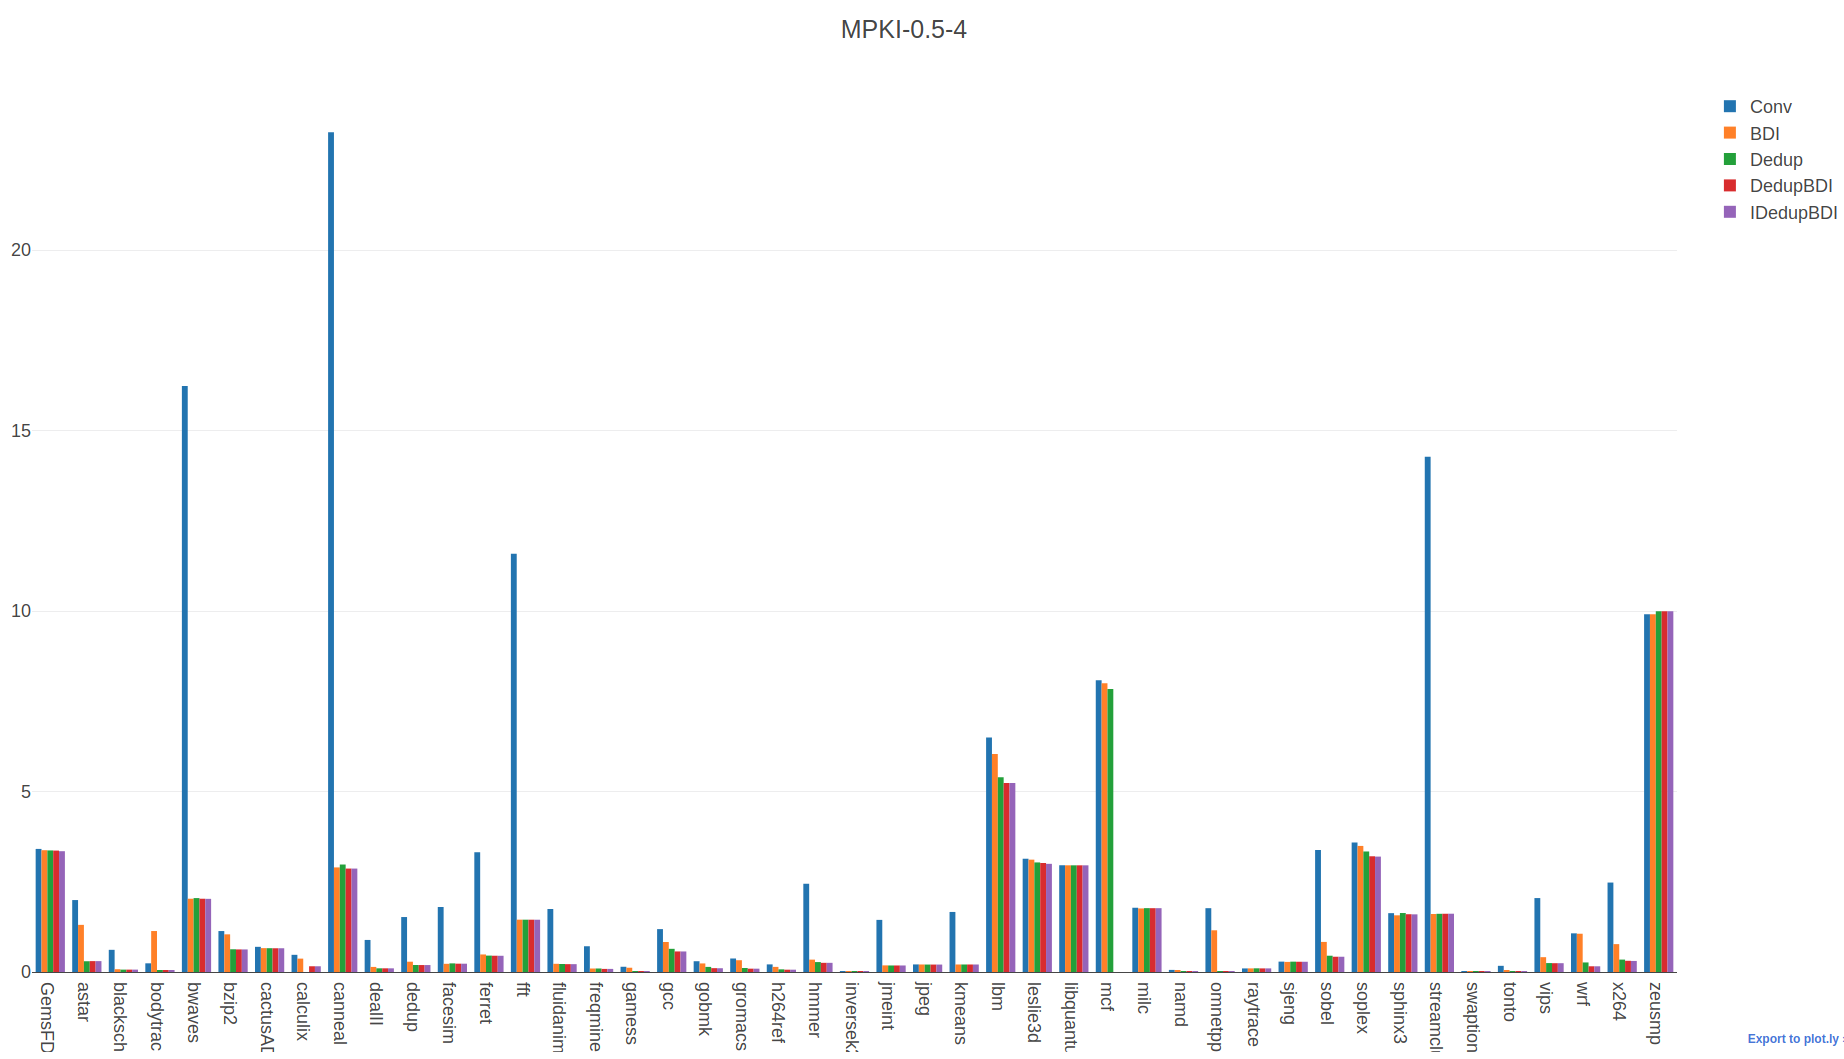
\includegraphics[width=\textwidth]{all05-mpki.png}
    \end{subfigure}
    \begin{subfigure}{\textwidth}
        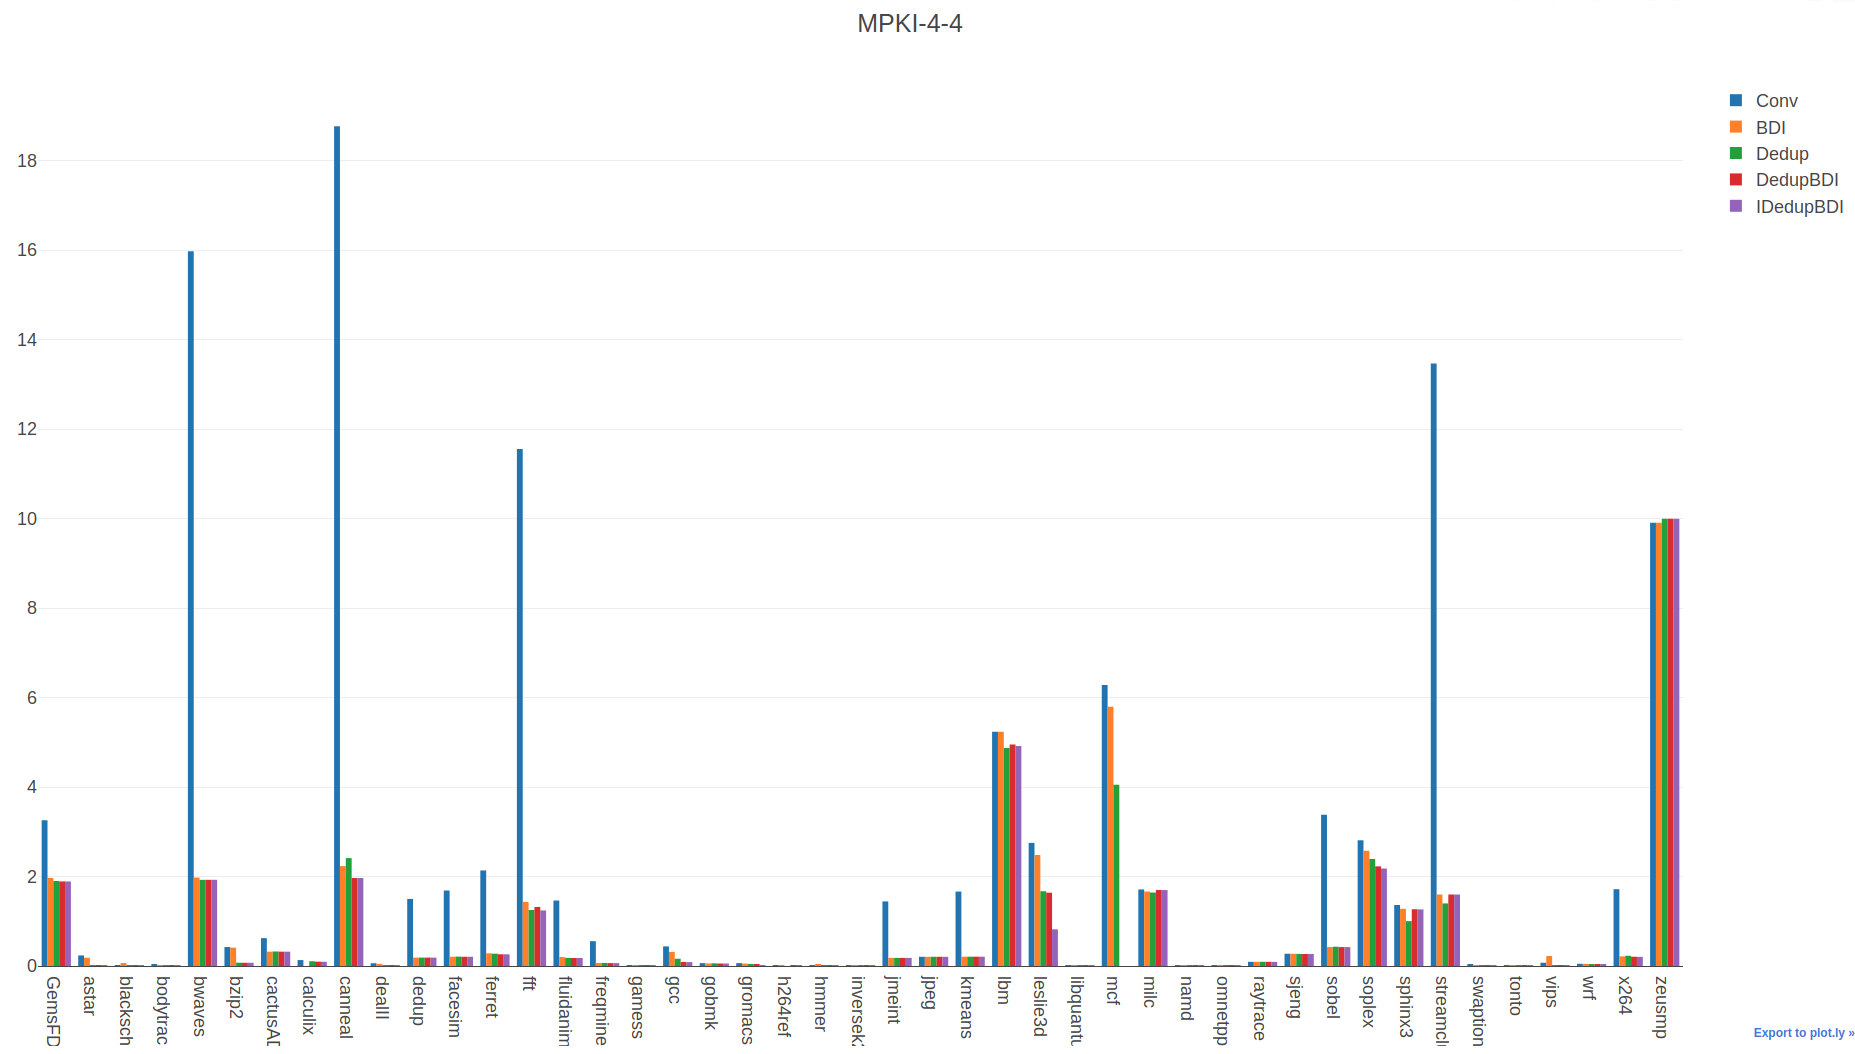
\includegraphics[width=\textwidth]{all4-mpki.png}
    \end{subfigure}
    \caption[All benchmarks: MPKI]{Showing LLC MPKI for conventional and all types of compressed 0.5 and 4MB caches with tags four times data.}
    \label{fig:all_mpki}
\end{figure}
\begin{figure}
    \begin{subfigure}{\textwidth}
        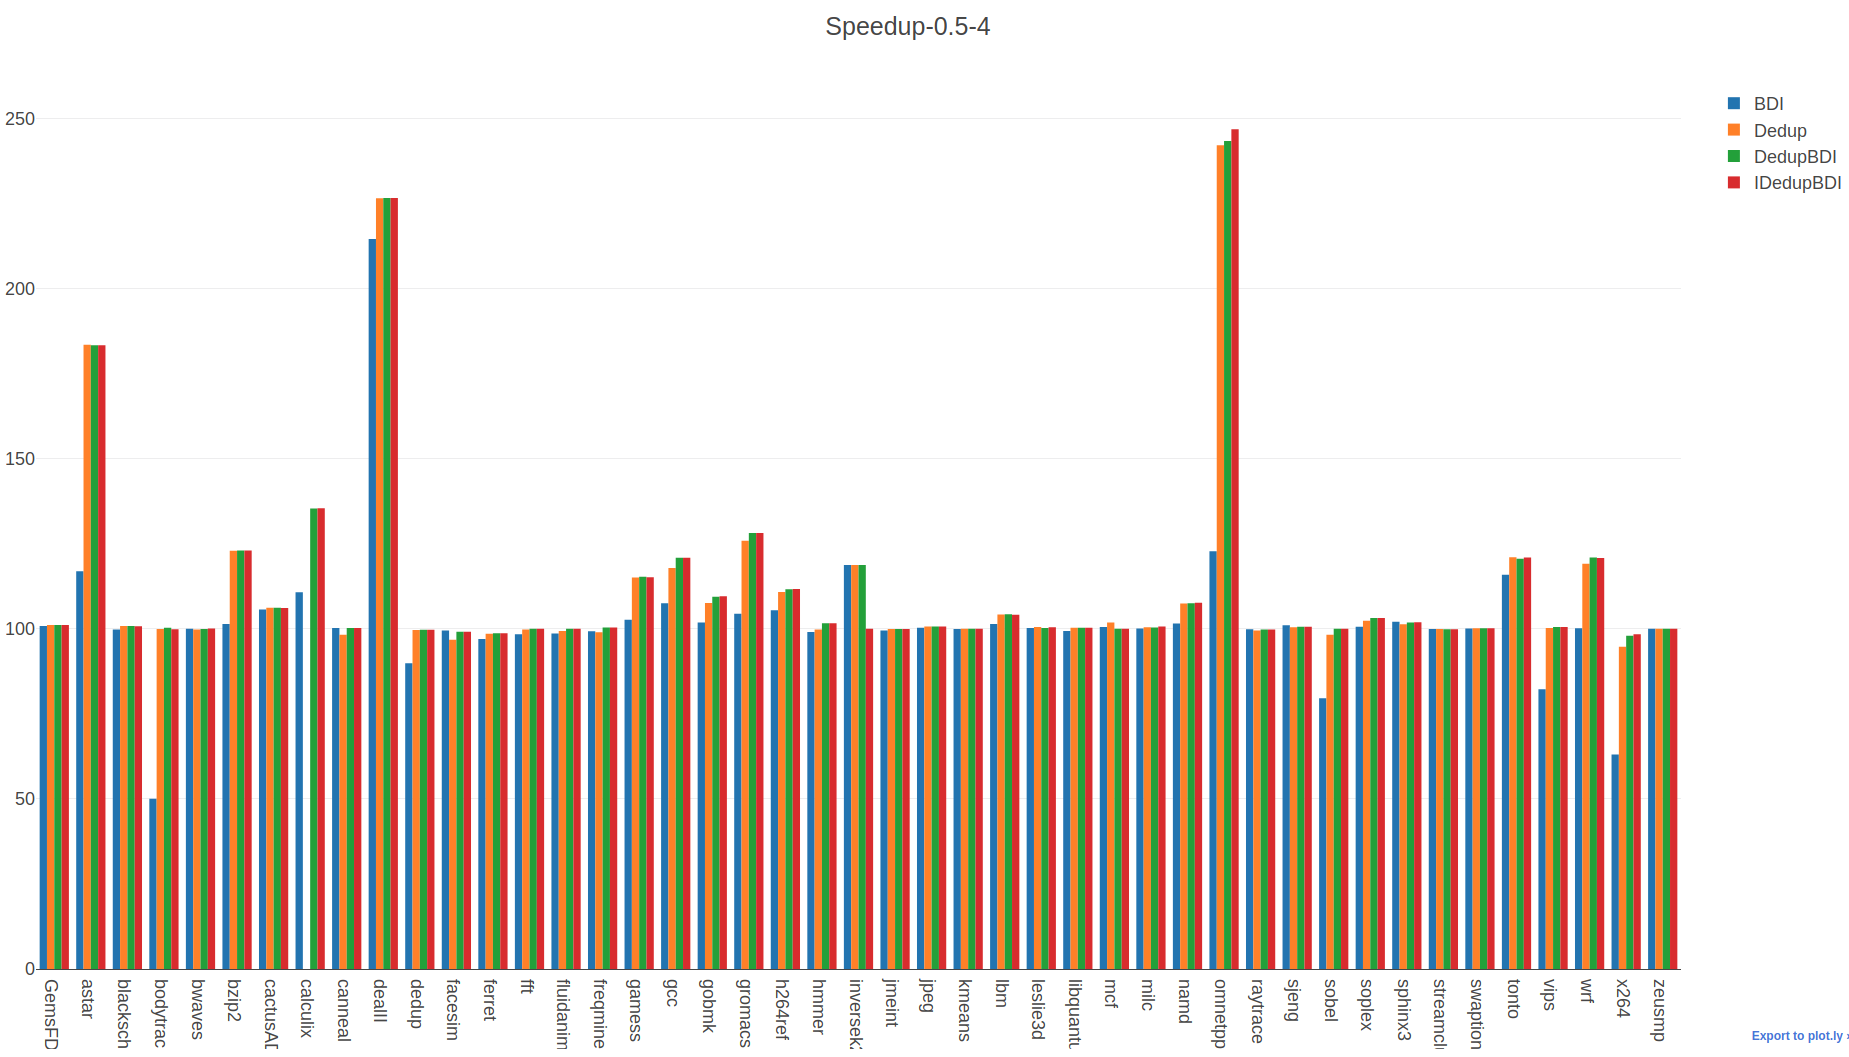
\includegraphics[width=\textwidth]{all05-speedup.png}
    \end{subfigure}
    \begin{subfigure}{\textwidth}
        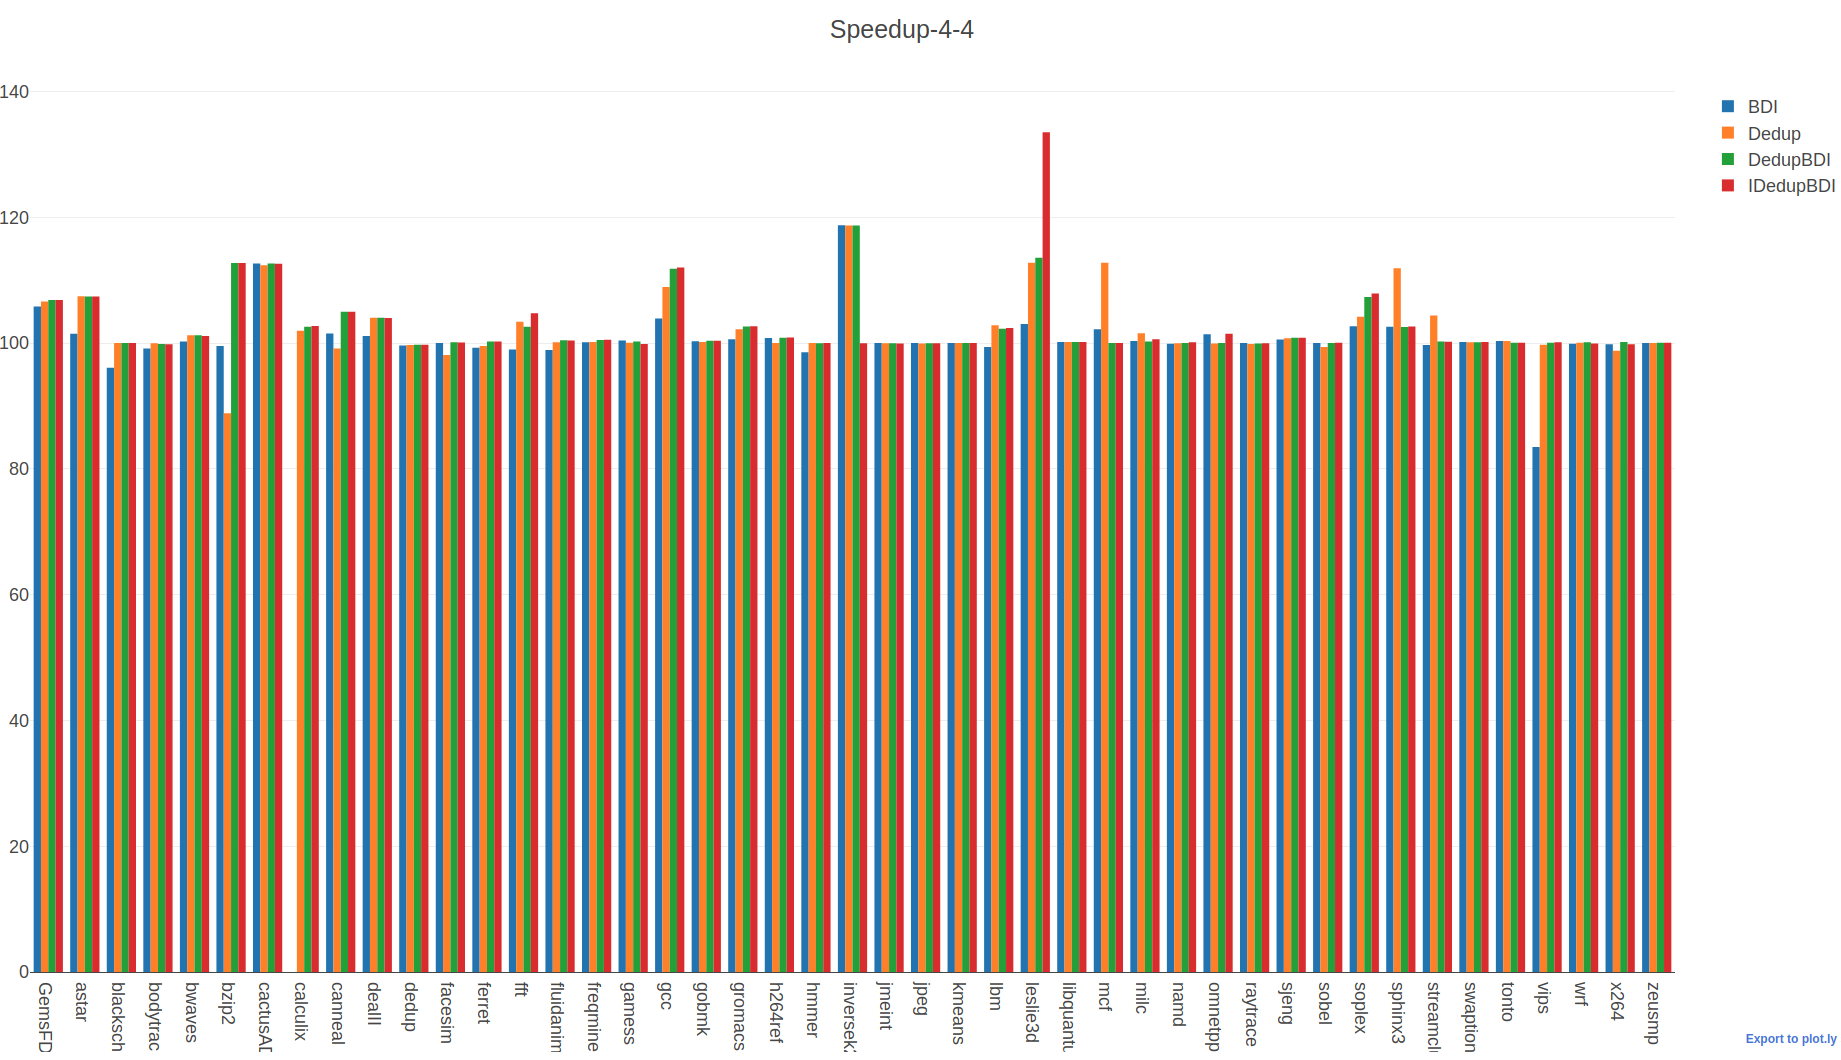
\includegraphics[width=\textwidth]{all4-speedup.png}
    \end{subfigure}
    \caption[All benchmarks: Speedup]{Showing Speedup for all types of compressed 0.5 and 4MB caches with tags four times data against conventional same size caches.}
    \label{fig:all_speedup}
\end{figure}
Figure \ref{fig:all_mpki} shows the MPKI for all the benchmarks when simulated with conventional and compressed 0.5MB and 4MB LLC caches with tags four times the data lines. It shows that compressed caches reduce MPKIs in LLC. DedupBDI is either the same as Dedup or BDI or is outperforming them.\par
However, the decrease of MPKI doesn't always necessitate speedup. The benchmark access patterns and cache sensitivity also play a role. Table \ref{tab:cachesense} shows the behavior of all benchmarks over a range fo cache sizes. Every benchmark is classified as cache sensitive, cache insensitive, or cache sensitive at a specific cache size range.
Figure \ref{fig:all_speedup} shows the speedup for all the benchmarks when simulated with a compressed 0.5MB and 4MB LLC caches with tags four times the data lines, respectively. We have chosen those two sizes because some benchmarks are only cache sensitive with lower cache sizes while others are only cache sensitive at higher cache sizes.\par
For the cache insensitive benchmarks, the DedupBDI cache performs as fast as the conventional caches. It does not provide anymore speedup. But it allows the data to be compressed, providing area and power savings. For the cache sensitive benchmarks, DedupBDI outperforms the conventional, Dedup, and DedupBDI caches altogether.

\section{Tag to Data Ratio}
\label{sec:tagratio}
\begin{figure}
    \begin{subfigure}{\textwidth}
        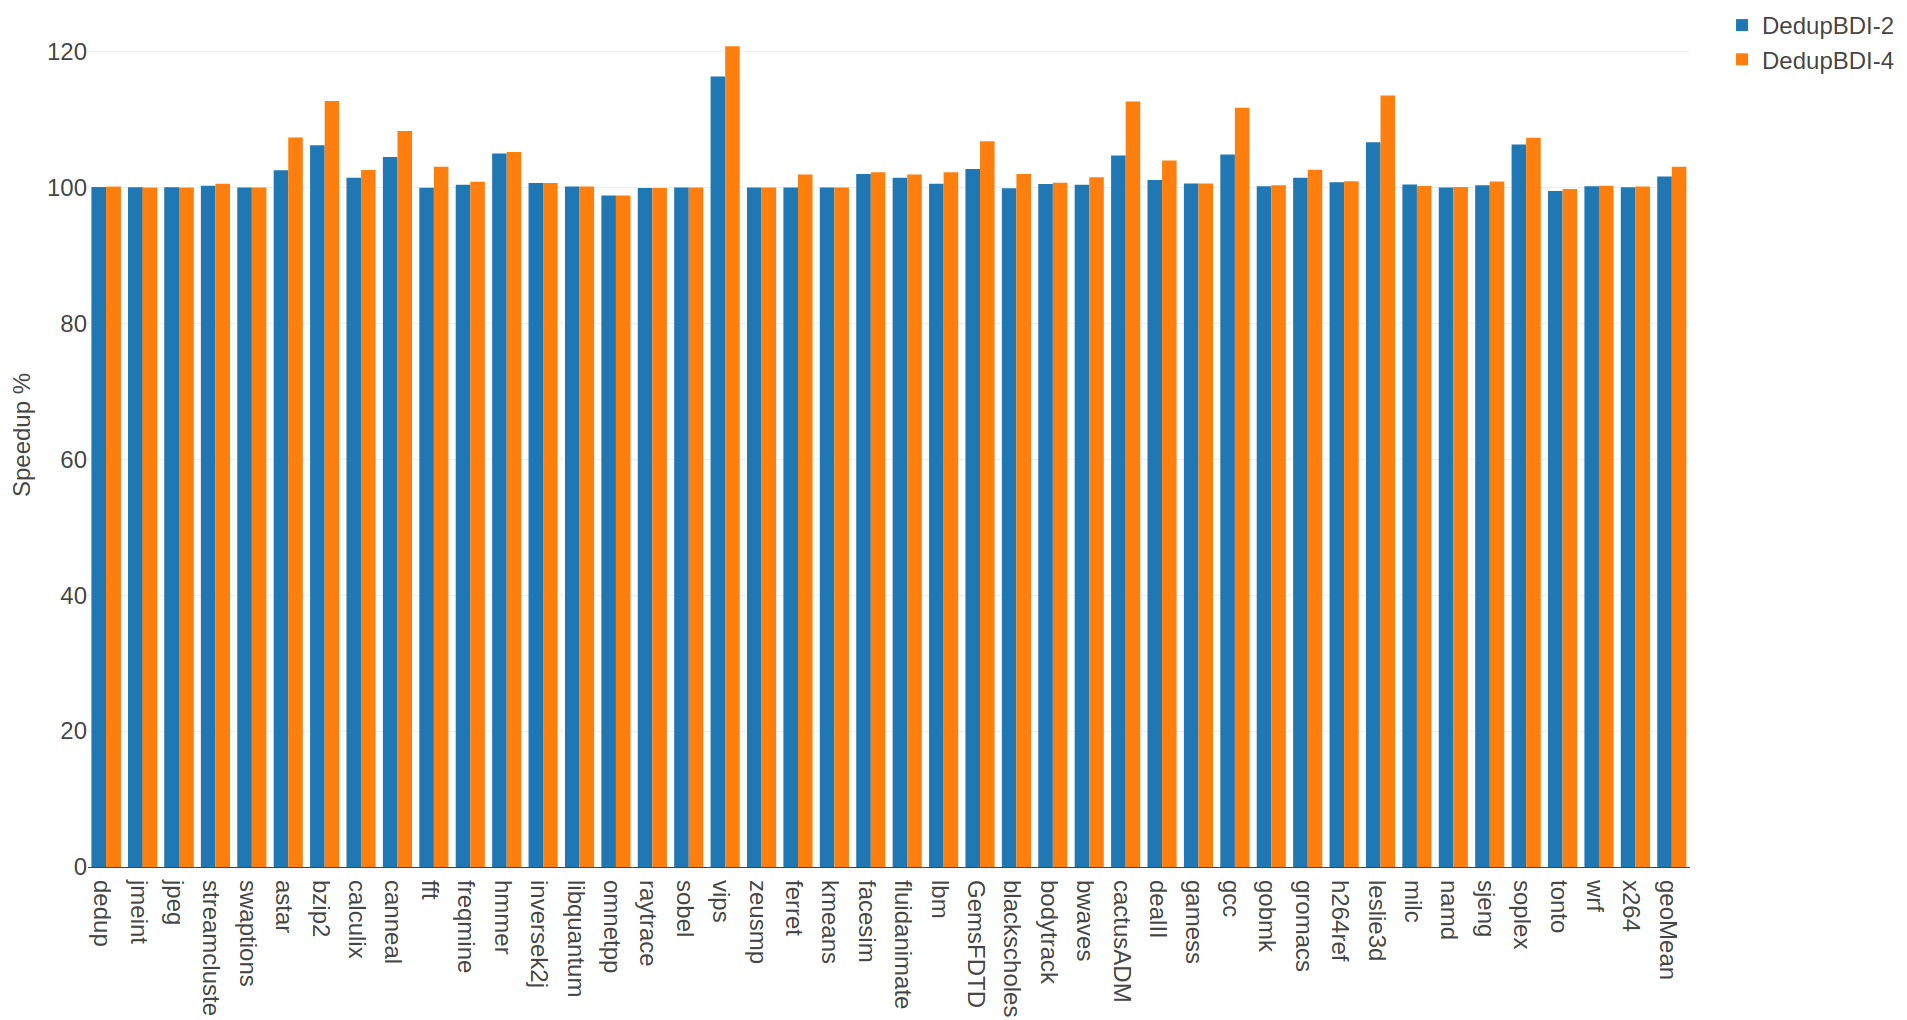
\includegraphics[width=\textwidth]{compare-speedup.png}
    \end{subfigure}
    \begin{subfigure}{\textwidth}
        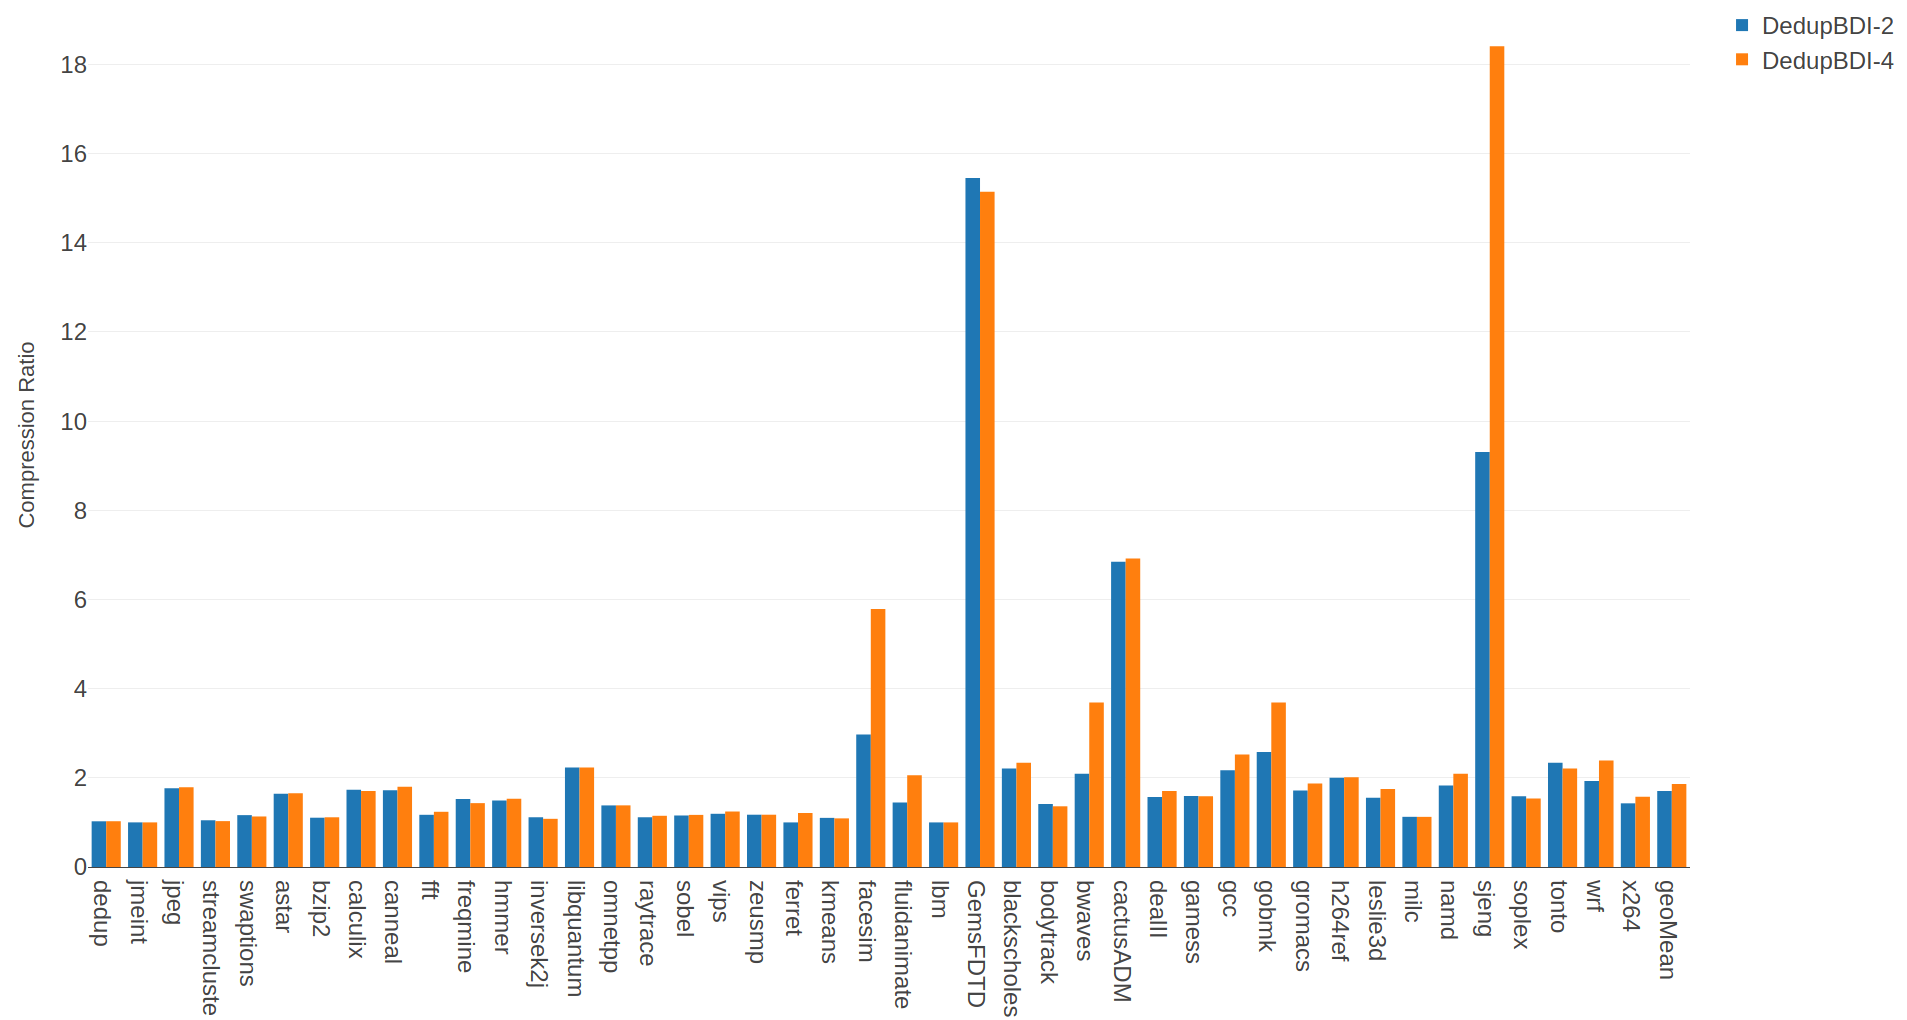
\includegraphics[width=\textwidth]{compare-compression.png}
    \end{subfigure}
    \caption[All benchmarks: Tag Ratio]{Showing performance and compression ratio for all benchmarks using DedupBDI 4MB caches with tags four times data and twice the data.}
    \label{fig:all_compare}
\end{figure}
Figure \ref{fig:all_compare} shows the difference between two 4MB DedupBDI caches, one with tags twice the data entries and the other with tags four times the entries. Using the tags as four times the data entries means the data array will be twice as small but it also requires compression to be highly effective. Otherwise the cache will run out of data space quickly and throttle the performance. As Figure \ref{fig:all_compare} shows, the smaller 4MB-4 cache achieves better performance than the 4MB-2 and has better compression ratio. We've chosen caches with four times the tags to be our default compressed cache size.


\section{Overhead Analysis}
\label{sec:Overhead}
\begin{table}[]
    \centering
    \begin{tabular}{lllll}
               & Conv   & BDI    & Dedup  & DedupBDI \\ \hline
    Tags       &        &        &        &          \\
    \# Entries & 8192   & 8192   & 8192   & 8192     \\
    Entry Size & 49b    & 49b    & 49b    & 49b      \\
    Overhead   & 6b     & 15b    & 35b    & 42b      \\
    Total Size & 55KB   & 64KB   & 84KB   & 91KB     \\ \hline
    Data       &        &        &        &          \\
    \# Entries & 8192   & 2048   & 2048   & 2048     \\
    Entry Size & 64B    & 64B    & 64B    & 64B      \\
    Overhead   &        &        & 11b    & 11B      \\
    FreeList   &        &        & 2.75KB & 896B     \\
    Total Size & 0.5MB  & 125KB  & 133.5KB & 150.875KB   \\ \hline
    Hash       &        &        &        &          \\
    \# Entries &        &        & 64     & 64       \\
    Entry Size &        &        & 10b    & 10b      \\
    Overhead   &        &        & 11b    & 14b      \\
    Total Size &        &        & 168B   & 192B     \\ \hline
    Total Bank Size & 567KB & 189KB & 217.6KB & 242KB  
    \end{tabular}
    \caption{4MB cache size and overhead in all configurations.}
    \label{tab:overhead}
\end{table}
Table \ref{tab:overhead} shows the overheads in one bank in the cache designs we have, assuming an 8 banked cache, with an associativity of 16, cache size of 4MB and LRU replacement policy. The overhead in all caches comes from three (four) different sources:
\begin{itemize}
    \item \textbf{Tag Overhead:}
    \begin{itemize}
        \item \textbf{conventional:} In conventional caches, assuming LRU replacement policy, the tag overhead per entry consists of one bit for Valid, one for Dirty, and log2(associativity) bits for the LRU replacement. 
        \item \textbf{BDI:} In BDI there's an extra overhead of 4 bits for compression encoding and log2(associativity*\#SegmentsPerLine) bits for segment pointers. Along with the normal overhead from a conventional cache. Note that in BDI the data array has half or one quarter of the associativity of the tag array.
        \item \textbf{Dedup:} On top of the conventional cache overhead, Dedup adds two pointers per tag entry for the next/previous tag to build a linked list, each one of those is log2(\#Tags/associativity) bits. It also adds pointers to the data line associated with it. Since Dedup data arrays are direct mapped the data pointer size is log2(\#Data).
        \item \textbf{DedupBDI:} DedupBDI adds the same overhead as the BDI cache. It also adds the same linked list pointers from the Dedup cache, but it's data pointer size is different from the Dedup cache. Because the data array in DedupBDI maintains its associativity, the data pointer size is log2(\#Data/associativity).
    \end{itemize}
    \item \textbf{Data Overhead:}
    \begin{itemize}
        \item \textbf{conventional:} A conventional cache has no overheads in its data array.
        \item \textbf{BDI:} Similar to a conventional cache, A BDI cache does not have any metadata in its data array and thus does not have any overhead.
        \item \textbf{Dedup:} The data lines in a Dedup cache requires a pointer to the tag, which is enough to pint to the tag set so it has a size of log2(\#Tags/associativity). It also requires each data line to have a deduplication counter, which we described in \ref{ch:BackgroundMotiv} to be 2 bits.
        \item \textbf{DedupBDI:} The DedupBDI data array has the same overhead as its Dedup counterpart. Except the overhead is per segment instead of being per line. that means for each data line we have 8 Dedup data overheads.
    \end{itemize}
    \item \textbf{Extra Data Overhead:}
    \begin{itemize}
        \item \textbf{Dedup:} The Dedup cache maintains a free list of its free data lines. The free list is essentially a FIFO with the same number of entries as data lines, and with a width that's enough to hold a pointer to the corresponding data line (i.e. log2(\#Data)).
        \item \textbf{DedupBDI:} The DedupBDI cache maintains 8 different free lists. Each of them is a FIFO with the same number of sets as data sets (i.e. Data lines/associativity), with a width that's enough to hold a pointer to the set (i.e. log2(\#Data/associativity)).
    \end{itemize}
    \item \textbf{Hash Array:} The Dedup and DedupBDI have the same hash array design. The hash array saves part of the hash as a tag while the other part is used as an index. The hash array then has the size of \#Hash*(HashSize-log2(\#Hash/associativity)). The Dedup and DedupBDI hash arrays then have some extra overhead:
    \begin{itemize}
        \item \textbf{Dedup:} each hash entry has a data pointer of size log2(\#Data)
        \item \textbf{DedupBDI:} each hash entry has a data pointer of size log2(\#Data/associativity) and segment pointer of size log2(associativity*\#SegmentsPerLine) bits.
    \end{itemize}
\end{itemize}
It's obvious that DedupBDI has the highest amount of overhead. But it also gains the most savings and speedups.

\section{Area and Power}
\label{sec:areapower}
\begin{table}[]
    \centering
    \resizebox{\textwidth}{!}{%
    \begin{tabular}{llllll}
    \multicolumn{2}{c}{Cache}                                                 & \multicolumn{1}{c}{\begin{tabular}[c]{@{}c@{}}Access Latency\\ (ns)\end{tabular}} & \multicolumn{1}{c}{\begin{tabular}[c]{@{}c@{}}Dynamic Read\\ Energy (nJ)\end{tabular}} & \multicolumn{1}{c}{\begin{tabular}[c]{@{}c@{}}Leakage Power\\ (mW)\end{tabular}} & \multicolumn{1}{c}{Area (mm2)} \\ \hline
    \multicolumn{1}{l|}{\multirow{5}{*}{CONV}}     & \multicolumn{1}{l|}{0.5} & 1.040842                                                                          & .28134914                                                                              & 353.32648                                                                        & 12.2026068                     \\
    \multicolumn{1}{l|}{}                          & \multicolumn{1}{l|}{1}   & 1.116541                                                                          & .29846783                                                                              & 530.37712                                                                        & 13.073461                      \\
    \multicolumn{1}{l|}{}                          & \multicolumn{1}{l|}{2}   & 1.285388                                                                          & .33135866                                                                              & 884.79016                                                                        & 14.771159                      \\
    \multicolumn{1}{l|}{}                          & \multicolumn{1}{l|}{4}   & 1.46331                                                                           & .3967712                                                                               & 1579.6440                                                                        & 18.129441                      \\
    \multicolumn{1}{l|}{}                          & \multicolumn{1}{l|}{8}   & 1.917741                                                                          & .526493                                                                                & 2978.4016                                                                        & 24.880933                      \\ \cline{1-2}
    \multicolumn{1}{l|}{\multirow{5}{*}{BDI}}      & \multicolumn{1}{l|}{0.5} & 1.010391                                                                          & .26910215                                                                              & 236.31936                                                                        & 11.605206                      \\
    \multicolumn{1}{l|}{}                          & \multicolumn{1}{l|}{1}   & 1.045793                                                                          & .27524057                                                                              & 298.75176                                                                        & 11.921437                      \\
    \multicolumn{1}{l|}{}                          & \multicolumn{1}{l|}{2}   & 1.126943                                                                          & .28691374                                                                              & 415.8200                                                                         & 12.527563                      \\
    \multicolumn{1}{l|}{}                          & \multicolumn{1}{l|}{4}   & 1.297986                                                                          & .3083546                                                                               & 655.4520                                                                         & 13.701536                      \\
    \multicolumn{1}{l|}{}                          & \multicolumn{1}{l|}{8}   & 1.385186                                                                          & .3511512                                                                               & 1130.4840                                                                        & 15.981861                      \\ \cline{1-2}
    \multicolumn{1}{l|}{\multirow{5}{*}{DEDUP}}    & \multicolumn{1}{l|}{0.5} & 1.026490                                                                          & .26946535                                                                              & 240.20488                                                                        & 11.623081                      \\
    \multicolumn{1}{l|}{}                          & \multicolumn{1}{l|}{1}   & 1.070838                                                                          & .27615777                                                                              & 310.98856                                                                        & 11.976806                      \\
    \multicolumn{1}{l|}{}                          & \multicolumn{1}{l|}{2}   & 1.156487                                                                          & .28876076                                                                              & 440.1304                                                                         & 12.642104                      \\
    \multicolumn{1}{l|}{}                          & \multicolumn{1}{l|}{4}   & 1.396239                                                                          & .3130041                                                                               & 714.2168                                                                         & 13.976212                      \\
    \multicolumn{1}{l|}{}                          & \multicolumn{1}{l|}{8}   & 1.481563                                                                          & .3610318                                                                               & 1263.6328                                                                        & 16.601801                      \\ \cline{1-2}
    \multicolumn{1}{c|}{\multirow{5}{*}{DEDUPBDI}} & \multicolumn{1}{l|}{0.5} & .971216                                                                           & .27016215                                                                              & 246.69448                                                                        & 11.655013                      \\
    \multicolumn{1}{c|}{}                          & \multicolumn{1}{l|}{1}   & 1.085028                                                                          & .27733513                                                                              & 324.34256                                                                        & 12.039511                      \\
    \multicolumn{1}{c|}{}                          & \multicolumn{1}{l|}{2}   & 1.172562                                                                          & .29132959                                                                              & 468.7792                                                                         & 12.778273                      \\
    \multicolumn{1}{c|}{}                          & \multicolumn{1}{l|}{4}   & 1.428335                                                                          & .3183339                                                                               & 773.8560                                                                         & 14.257854                      \\
    \multicolumn{1}{c|}{}                          & \multicolumn{1}{l|}{8}   & 1.522417                                                                          & .3725894                                                                               & 1392.7656                                                                        & 17.212904                      \\ \cline{1-2}
    \end{tabular}%
    }
    \caption{Area, Power, Energy, and Access Latency for all cache sizes and configurations.}
    \label{tab:areapower}
\end{table}
We used cacti6\cite{cacti} to get power and area estimations for all the cache types and sizes we simulated. The results are shown in \ref{tab:areapower}. The results in the table are consistent with what we've discussed so far. Compressed caches have lower access latencies, energy and power consumption than their conventional counterparts because of their lesser size. With DedupBDI consuming the most resources out of the compressed caches. The extra resources however are justified as they allow better speedup and compression.